%%
%% Copyright 2019-2021 Elsevier Ltd
%% 
%% This file is part of the 'CAS Bundle'.
%% --------------------------------------
%% 
%% It may be distributed under the conditions of the LaTeX Project Public
%% License, either version 1.2 of this license or (at your option) any
%% later version.  The latest version of this license is in
%%    http://www.latex-project.org/lppl.txt
%% and version 1.2 or later is part of all distributions of LaTeX
%% version 1999/12/01 or later.
%% 
%% The list of all files belonging to the 'CAS Bundle' is
%% given in the file `manifest.txt'.
%% 
%% Template article for cas-dc documentclass for 
%% double column output.

\documentclass[a4paper,fleqn]{cas-dc}

% If the frontmatter runs over more than one page
% use the longmktitle option.

%\documentclass[a4paper,fleqn,longmktitle]{cas-dc}

\usepackage[numbers]{natbib}
%\usepackage[authoryear]{natbib}
%\usepackage[authoryear,longnamesfirst]{natbib}

\usepackage{graphicx}
\usepackage{amsmath}
\usepackage{algorithm}
\usepackage{algorithmic}
\usepackage{xurl}
\hyphenation{op-tical net-works semi-conduc-tor}

\usepackage{todonotes}
\graphicspath{ {./figures/} }
\usepackage{subcaption}
\usepackage{booktabs}
\usepackage{siunitx}
\sisetup{round-mode=places, round-precision=2}
\usepackage{enumitem}

\usepackage{soul}

\newcommand{\blindtext}[1]{\textbf{$<<$Text hidden for blind review$>>$}}
\newcommand{\sergio}[1]{\textcolor{black}{#1}}
\newcommand{\mm}[1]{\textcolor{black}{#1}}
\newcommand{\review}[1]{\textcolor{blue}{#1}}

\usepackage[percent]{overpic}
\usepackage[super]{nth}
\usepackage{pdfpages}
\usepackage{multirow}

\DeclareUnicodeCharacter{2009}{\,}

\begin{document}

\let\WriteBookmarks\relax
\def\floatpagepagefraction{1}
\def\textpagefraction{.001}

% Short title
\shorttitle{MPI Malleability Validation under HPC Conditions}    

% Short author
\shortauthors{S. Iserte et al.}  

\title [mode = title]{MPI Malleability Validation under Replayed Real-World HPC Conditions}


\author[1]{Sergio Iserte}[orcid=0000-0003-3654-7924]
\ead{sergio.iserte@bsc.es}
\cormark[1]
\cortext[1]{Corresponding author}

\author[2]{Maël Madon}[orcid=0000-0001-9476-4682]
\author[2]{Georges Da~Costa}[orcid=0000-0002-3365-7709]
\author[2]{Jean-Marc Pierson}[orcid=0000-0001-8948-0474]
\author[1]{Antonio J. Peña}[orcid=0000-0002-3575-4617]

\affiliation[1]{organization={Barcelona Supercomputing Center (BSC)},
            %addressline={}, 
            city={Barcelona},
            %citysep={}, % Uncomment if no comma needed between city and postcode
            %postcode={08034}, 
            % state={},
            country={Spain}}
            
\affiliation[2]{organization={University of Toulouse, CNRS, Toulouse INP, IRIT},
            % addressline={}, 
            city={Toulouse},
            % citysep={}, % Uncomment if no comma needed between city and postcode
            %postcode={12071}, 
            % state={},
            country={France}}

% Corresponding author text
%\cortext[1]{Corresponding author}

% Footnote text
%\fntext[1]{}

% For a title note without a number/mark
%\nonumnote{}

% Here goes the abstract
\begin{abstract}
Dynamic Resource Management (DRM) techniques can be leveraged to maximize throughput and resource utilization in computational clusters.
Although DRM has been extensively studied through analytical workloads and simulations, skepticism persists among end administrators and users regarding their feasibility under real-world conditions.
To address this problem, we propose a novel methodology for validating DRM techniques, such as malleability, in realistic scenarios that reproduce actual cluster conditions of jobs and users by replaying workload logs on a High-performance Computing (HPC) infrastructure.
Our methodology is capable of adapting the workload to the target cluster.
We evaluate our methodology in a malleability-enabled 125-node partition of the Marenostrum~5 supercomputer. Our results validate the proposed method and assess the benefits of MPI malleability on a novel use case of a pioneer user of malleability (our ``PhD Student''): parallel-efficiency-aware malleability reduced a malleable workload time by 27\% without delaying the baseline workload, although introducing queueing delays for individual jobs, but maintaining the resource utilization rate.
\end{abstract}

% Use if graphical abstract is present
%\begin{graphicalabstract}
%\includegraphics{}
%\end{graphicalabstract}

% Keywords
% Each keyword is seperated by \sep
\begin{keywords}
\sep Dynamic Resource Management
\sep Replay with Feedback
\sep Malleability
\sep Workload Characterization
\sep Cluster Computing
\end{keywords}

\maketitle

\section{Introduction}\label{intro}
High-performance computing (HPC) facilities are critical for advancing scientific research, engineering, and data analysis across various domains, from genomic research~\cite{martinez_dynamic_2013, zhong_gpu_2025} to multi-physics simulations~\cite{hess_gromacs_2008, vazquez_alya_2016, caviedes-voullieme_serghei_2023} through artificial intelligence~\cite{martinez-cuenca_use_2023, rosciszewski_optimizing_2023, godoy_large_2024}. 
These computational clusters rely on efficiently utilizing resources to maximize their productivity. Dynamic resource management (DRM) techniques have emerged as key strategies to improve the utilization of these systems~\cite{bungartz_invasive_2013, garcia_hints_2014, lopez_openmp_2021}. These techniques enable the flexible allocation and reallocation of computational resources and reconfiguring jobs accordingly to adapt to the dynamic nature of HPC workloads.
Among others, malleability based on the Message-Passing Interface (MPI) is one of the most extended DRM approaches to process layout reshape and data redistribution
~\cite{10.1145/3555819.3555856, iserte_agut_high-throughput_2018, martin_flex-mpi_2013, bhattarai_dynamic_2024}.

Despite their potential, DRM techniques face several challenges that hinder their adoption in production environments~\cite{iserte_resource_2025}.
Particularly, MPI malleability requires 1) a malleability-ready resource management system (RMS), which many existing facilities do not possess, and 2) a malleability framework to develop malleable applications compatible with the RMS and the available distributed parallel runtime systems in the cluster.
These kinds of limitations increase the complexity of evaluating DRM techniques with realistic workloads and foster skepticism among end users and system administrators regarding DRM's practical benefits and feasibility.
In this regard, previous studies evaluating DRM techniques have relied on simplistic simulations, biased benchmarks, or synthetic traces, often failing to accurately represent real-world systems' conditions. These analytic workloads do not capture the variability and unpredictability of user behaviors observed in production systems. As a result, researchers in this field have faced challenges in conducting impactful demonstrations that significantly influence the community (more details in Section~\ref{sec:related}).

To address the challenges of evaluating DRM techniques, we propose a novel methodology that leverages supercomputer logs to generate realistic workloads based on actual user submission behaviors, including temporal patterns across hours and days of the week. Our approach introduces a mechanism called the \textit{User-Based Submitter}, designed to scale across different computing clusters. Rather than relying on synthetic simulations, this method replays real user interactions from production supercomputers, enabling a more accurate and comprehensive evaluation of DRM techniques.

We further incorporate malleable jobs into these replayed workloads to assess the impact of DRM on job execution and system performance. This allows us to observe the effects of job malleability and resource reallocation in a controlled yet realistic environment. Notably, the study includes the perspective of a pioneering user—submitting the first malleable jobs in a 125-node partition—demonstrating the potential of our methodology to validate previous findings and uncover new insights in real HPC settings. It is worth noting that the cluster size used in our experiments ranks among the largest evaluated in state-of-the-art malleability studies (see Section~\ref{sec:related}).

In summary, this paper presents 
1) \textbf{a methodology to replay logs in any computational cluster keeping the logic behind user submissions}. 
Instead of a mathematical model, this methodology uses the techniques of user sampling from a recorded log and replay with feedback to reproduce the workload in a target system (see Section~\ref{sec:methodology}).
This paper particularly 
2) \textbf{designs and analyzes a novel case study of the adoption of malleability in a production system}. For this purpose, the authors exemplify this event with a new user (``the student'') who is the pioneer in submitting malleable jobs to the cluster. Among all the possible scenarios, the authors have decided to develop a case that paves the way to more complex malleable workloads (see Section~\ref{sec:experiments}).
Similarly to hardware simulators that have to be validated in actual hardware to be published, this paper presents, for the first time in the literature, 
3) \textbf{the validation of MPI malleability using a real workload in a malleability-enabled supercomputer}, without simulations or synthetic benchmarks (see Section~\ref{sec:results}). 

The paper ends with a discussion of the applicability of the presented technique and the meaningful results obtained in the evaluation of the validation methodology (see Section~\ref{sec:discussion}). It concludes with a summary of our contributions and findings (see Section~\ref{sec:conclusion}).

\section{Related Work}\label{sec:related}
This section reviews the previous efforts done in the fields of workload replay and dynamic resource management.

\subsection{Workload Replay}
A classical approach to evaluate resource management policies consists of replaying a historical workload from its log.
However, modifying the target infrastructure or scheduling policies impacts the system's performance (e.g., response time, computing speed, resource availability),
which has a crucial impact on the submission behavior of its users~\cite{zakay_preserving_2014, schlagkamp_influence_2017}.
As a result, many previous works in the field have generalization issues, since they do not account for these behaviors.
A solution is to perform closed-loop simulations~\cite{schroeder_open_2006},
where the submitted workload adapts to the simulated performance of the system.
To do so, the authors in~\cite{zakay_identifying_2013} extract relevant submission patterns from historical workloads to replay them in simulations.
More recently, the authors in~\cite{madon_replay_2024} provide an in-depth study of this technique, named ``replay with feedback''.
In~\cite{feitelson_resampling_2021}, the authors go one step further and suggest using \emph{resampling} with feedback for performance evaluation where the historical workload is scaled to the target infrastructure through user sampling.

\subsection{Dynamic Resource Management}
The MPI paradigm is the {\it de facto} standard for implementing distributed parallel applications designed to run on computational clusters. MPI provides efficient and straightforward mechanisms for communication among different processes, known as ranks, each with its own memory address space.
In a traditional MPI job, a fixed number of ranks are initiated at the start and remain active until the completion of the job. This static allocation of resources may lead to inefficiencies, especially in dynamic and heterogeneous computing environments.

MPI malleability addresses these inefficiencies through DRM. This technique allows the number of MPI ranks to be modified during the execution of a program, enabling the application to resize on the fly~\cite{feitelson_packing_1996}. Malleable MPI applications may adapt to changing computational resources, improving overall system utilization and application performance.
Although MPI malleability could be seen as a variant of checkpoint/restart, most modern solutions implement on-memory data redistribution, reducing overheads from accessing storage media.

Closely related to malleability is the concept of moldability. While malleability involves adjusting the number of MPI ranks during the execution of a job, moldability determines the number of ranks at the time of job submission before its initialization~\cite{lublin_workload_2003}. 
In this regard, jobs specify a range of sizes, allowing the job scheduler to choose the most suitable configuration based on current system availability and load.
This approach provides an extra degree of flexibility by enabling better resource allocation at job scheduling time, which can lead to improved system efficiency and potentially shorter wait times for job initiation. However, unlike malleable applications, moldable applications do not adjust their resource usage dynamically during runtime.

Surveys in ~\cite{aliaga_survey_2022, Tarraf_malleability_2024} extensively review the state--of--the--art of malleability in HPC systems. Instead, we focus on how malleability frameworks and actual RMSs have been evaluated with workloads to demonstrate the usefulness of DRM in clusters.

ReSHAPE is a coupled solution for adaptive workloads, including its specific reconfiguration libraries, scheduler, and runtime system.
This strong integration forces ReSHAPE users to develop applications that are compatible with this system.
In~\cite{sudarsan_reshape_2007}, ReSHAPE is evaluated in a 50-node cluster with a 5-job workload composed of the benchmarks LU, MM, Master-worker, Jacobi, and FFT, submitted simultaneously.
A subsequent publication added to the workload job instances of a malleable version of LAMMPS~\cite{sudarsan_dynamic_2009}.

PARM (acronym of Power-Aware Resource Manager) relies on over-provisioning, power capping, and job malleability, based on CHARM++ and Slurm~\cite{sarood_maximizing_2014}.
PARM is evaluated in a 38-node cluster with a 5-job workload comprising the benchmarks and applications Wave2D, Jacobi2D, LeanMD, Lulesh, and AMR.
Larger experiments relied on the Slurm simulator with a log of 68,936 jobs submitted to a 40,960-node cluster. The authors assume that all the jobs in the workload are malleable and assign them random scalability from a set of samples.

The solution developed by Prabhakaran et al. combines AMPI (based on CHARM++) with the RMS Torque/Maui to tackle malleable jobs~\cite{prabhakaran_batch_2015}. 
The authors evaluate in a 15-node cluster a workload based on a modified version of the ESP benchmark to contain various percentages of rigid, malleable, and evolving jobs composed of 230 instances.
While the rigid jobs followed the benchmark directives, the flexible jobs were a malleable version of LeanMD and an evolving implementation of the synthetic Quadflow.

The Dynamic Management of Resources Library (DMRlib) (detailed in Section~\ref{subsec:dmr}) was evaluated in a 129-node cluster with four benchmarks and applications (CG, Jacobi, N-Body, HPG-Aligner~\cite{iserte_dynamic_2019}) instantiated in 2,000-job workloads with various percentages of malleable jobs and turning on and off malleability in the applications of the workloads~\cite{iserte_dmrlib_2020}.
The authors leveraged the Feitelson synthetic workload generator~\cite{feitelson_towards_1996} to evaluate job scheduling algorithms in HPC.
This generator provides a way to simulate job arrival patterns, job sizes, and resource demands based on empirical data from real-world systems.

%In summary, prior research in this field has explored the effects of DRM using approaches ranging from benchmarks to simulations, often relying on artificially generated workloads that arbitrarily set job scales and submission patterns (e.g., steady or bursty).

%In contrast, with this research, we aim to validate past and future synthetic setups and results obtained for dynamic resource management replaying actual behaviors of users which are extremely difficult to be modeled with a mathematical function.

While prior research has explored the potential of DRM through benchmarks and simulations, these studies often rely on synthetic workloads with arbitrarily defined job sizes and submission patterns—such as steady or bursty arrivals—that fail to capture the complexity and variability of real-world HPC usage. These simplified models limit the generalizability and applicability of the findings to production systems.

In contrast, our work introduces a methodology that replays actual user behavior extracted from supercomputer logs, preserving the nuanced temporal and structural characteristics of real workloads. This approach enables the validation of past and future synthetic setups and their results, overcoming the limitations of synthetic modeling where user behavior is too complex to be accurately captured by mathematical functions. By grounding the evaluation in real-world conditions, we aim to bridge the gap between simulation-based studies and practical deployment in HPC infrastructures.

%In contrast, this work introduces a more robust methodology, leveraging user sampling and workload replay with feedback. Using a workload log from the Parallel Workload Archive\footnote{\url{https://www.cs.huji.ac.il/labs/parallel/workload}}, we adapt, fit, and replicate its activity on a malleability-enabled supercomputer partition. Additionally, we introduce a user periodically running malleable scientific applications based on a defined behavioral pattern.

%Out of the infinite cases that can be studied and given the current limitations of DRM integration in supercomputers, our study focuses on a practical scenario where infrastructure progressively adopts MPI malleability through a specific user with defined duties and deadlines. This scenario has not been previously studied in the literature.

\section{Methodology}\label{sec:methodology}

In order to study DRM under real-world conditions,
our method consists of reproducing the nominal activity of a cluster computing infrastructure.
We use a workload submitter based on the logic of users (Section~\ref{subsec:submitter}).
\sergio{The nominal activity is represented by submitting non-malleable jobs.}
These jobs, later called ``baseline workload'', are reproduced from historical workload logs and sized to our testbed through user sampling (Section~\ref{subsec:sampling}).
To study the effects of DRM on top of the baseline workload, the submitter includes an additional user leveraging moldability and malleability in her jobs, thanks to a malleable runtime (Section \ref{subsec:dmr}).

\iffalse
\begin{table}[tbp]
    \centering
    \begin{tabular}{lll}
        \toprule
         & \textbf{baseline workload} & \textbf{student workload} \\
         \midrule
         \textbf{origin} & historical workload & synthetic \\
         \textbf{UBS user type} & traditional & generative \\
         \textbf{replay method} & original timestamps & submit with feedback \\
         \textbf{job type} & mock MPI job & real MPI job \\
         \textbf{malleability enabled?} & no & yes \\
         \bottomrule
         
    \end{tabular}
    \caption{Summary characteristics of the two workloads submitted simultaneously in the cluster}
    \label{tab:my_label}
\end{table}
\fi

\subsection{User-Based Workload Submitter}
\label{subsec:submitter}

The core of the experiments presented in this paper relies on a piece of software running throughout the whole experiment duration: the User-Based Submitter (UBS)\footnote{Code available at \url{https://gitlab.bsc.es/siserte/ubs}}.%https://gitlab.irit.fr/sepia/coop/replay-on-rjms/poc}}.
UBS reproduces HPC users issuing job submissions to the Slurm resource manager at certain timestamps.
%\todo{Maël@IRIT: make an illustration?}
% the two types of users, the UBS, submitting jobs to SLURM
There are two types of users as described below:
\begin{itemize}[wide]
    \item \textit{Traditional users} submit jobs whose execution time, number of parallel resources, and submission time are given in an input file, based on a historical workload.
    These are used to replay the baseline workload.
    Consequently, the submitted jobs replicate the traditional rigid workload, allocating the requested resources during the desired time.

    \item \textit{Generative users} submit malleable jobs, using feedback on the status of previous submissions to decide on the following job submissions (see \cite{madon_replay_2024}).
    More precisely, a generative user takes as input a triplet $(t_0, \Delta t, N)$
    with $t_0$ the timestamp of their first submission,
    $\Delta t$ the think time between the end of the previous job and the submission of the new job and $N$ the total number of submissions from this user.
    %These are used to emulate the additional user, leveraging malleability and moldability.
    %The submitted jobs are actual instances of scientific parallel applications.
\end{itemize}

In the UBS, traditional and generative users are managed in two dedicated threads. 
The thread managing the traditional users sleeps until the next submission time, then calls a shell script issuing the job submission, passing it all relevant parameters about the job (i.e.: type, duration, or number of resources).
The thread of the generative users uses a socket to be informed of the completion of previous jobs. 
When a job owned by a generative user terminates, a new thread is started, sleeping for $\Delta t$ seconds before calling the submission script.

\subsection{User Sampling}
\label{subsec:sampling}

\renewcommand{\algorithmicrequire}{\textbf{Input:}}
\renewcommand{\algorithmicensure}{\textbf{Output:}}

\begin{figure*}[tbp]
  \centering
  \begin{minipage}{.6\linewidth}
    \begin{algorithm}[H]
      %\large
    \caption{User sampling from workload}\label{alg:sampling}
    \begin{algorithmic}[1]
        \REQUIRE $\bar{m} =$ the target median/average load per day
        \REQUIRE $M =$ the number of nodes in the target platform

        \STATE $U \leftarrow$ list of users in the workload
        \STATE $pool \leftarrow \{\}$, $m \leftarrow 0$
        % \STATE users.shuffle()
        \WHILE{$m \notin [.9\bar{m}, 1.1\bar{m}]$}
            \STATE $u \leftarrow$ draw a random user from $U$, without replacement 
            \IF{$max($nodes required by $u) < M$}
                \STATE $pool$.add($u$)
                \STATE $m \leftarrow$ load per day from users in $pool$
                \IF{$m > 1.1\bar{m}$}
                    \STATE $pool$.remove($u$)
                    \STATE $m \leftarrow$ load per day from users in $pool$
                \ENDIF
            \ENDIF
        \ENDWHILE
        \IF{$m \notin [.9\bar{m}, 1.1\bar{m}]$}
            \STATE print("SAMPLING FAILED!")
        \ENDIF

        \ENSURE $pool$
    \end{algorithmic}

    \end{algorithm}
  \end{minipage}
\end{figure*}

To create a realistic baseline workload of the actual activity in a cluster platform,
we leverage historical workload logs.
The challenge is to adapt this workload to the size of our testbed
\textit{without losing the logic of submission of the original users}.
Thus, instead of randomly sampling jobs from the original log,
we rather perform a sampling of \textit{users}, 
proceeding as described below (see Algorithm~\ref{alg:sampling}). 

First, we choose a target level of activity for the platform,
in terms of average or median load submitted per day.
For example, if the testbed has 100 nodes and we target 85\% activity,
we want the baseline workload to have approximately $85\times 24$ node-hours per day.
To reach the level, we proceed iteratively by randomly adding users to a user pool.
At each step, we calculate the load submitted daily by the users in the pool
by summing the product of execution time and number of nodes for all jobs submitted by these users in the original log.
If the activity reaches the desired level, the process is stopped; 
otherwise, we add a new user.
The last added user may overshoot the target;
in this case, that user is removed from the pool before adding another.

\subsection{Dynamic Resource Management}\label{subsec:dmr}

\begin{figure*}
\centering
    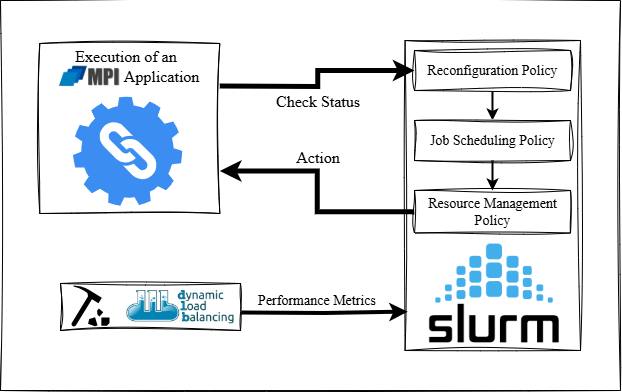
\includegraphics[clip,width=0.8\linewidth,trim={1.2cm 1.2cm 1.2cm 0.25cm}]{figures/dmr-slurm2.png}
    \caption{DMRlib Application--MPI--Slurm communication.}
    \label{fig:dmr-slurm}
\end{figure*}

This research enables DRM by leveraging moldability and malleability thanks to the Dynamic Management of Resources Library (DMRlib)~\cite{iserte_dmrlib_2020}.
DMRlib is a high-level API that facilitates the adoption of malleability in HPC codes. 
DMRlib implements a communication layer between the parallel distributed runtime (PDR) and the RMS, driving the management of processes and resources transparently to the user while providing flexibility to increase productivity and resource utilization of HPC facilities.

Figure~\ref{fig:dmr-slurm} depicts the operation of dynamic resource management in DMRlib, which is described as follows:

\begin{itemize}
\item During execution, jobs periodically expose their readiness for reconfiguration to the RMS.
\item This communication occurs at a synchronization point specified in the code, where the reconfiguration process may commence. In iterative applications, the end of an iteration often serves as an ideal synchronization point.
\item The RMS, with its cluster-wise information and the performance metrics provided by a monitor, determines reconfiguration actions following its defined policies, and informs the PDR.
\item If this results in a change to the job size, the RMS reallocates resources and returns the new number of processes, which may involve either expanding or shrinking the job.
\item Finally, the PDR redistributes the data among the processes according to the application's guidelines, allowing jobs to continue execution with the new process layout from the point where the reconfiguration was triggered.
\end{itemize}

\review{
DMRlib supports multiple Process Dynamic Runtimes (PDRs), including Nanos++~\cite{iserte_dmr_2018} and several MPI implementations~\cite{iserte_malleable_2025}, and can seamlessly interface with different malleability backends such as Proteo~\cite{martin-alvarez_proteo_2024} and DPP~\cite{huber_bridging_2025}.
}

In this work, DMRlib has been configured with MPICH\footnote{\url{https://www.mpich.org}}, as the PDR, and Slurm\footnote{\url{https://slurm.schedmd.com}} as the RMS~\cite{iserte_towards_2025}.
DMRlib integrates a monitoring module to track performance metrics during job execution and react accordingly by requesting/suggesting expansion or shrinking actions to the RMS.
Metrics are gathered by TALP~\cite{lopez_talp_2021}, which collects ``POP metrics''\footnote{\url{https://pop-coe.eu/node/69}}. This set of metrics is organized hierarchically and is multiplicative; that is, the value of the parent metric is equal to the product of the child metrics.
Among others, Parallel Efficiency (PE) reveals the inefficiency in splitting computation over processes and then communicating data among processes.
PE is a compound metric whose components reflect two critical factors to attain good parallel performance by ensuring even distribution of computational work across processes (load balance) and minimizing time communicating data among processes (communication efficiency).

%\sergio{
%DMRlib has proven to be a competitive dynamic resource management tool by its various published %success stories, such as~\cite{iserte_towards_2024}, recipient of the Best Paper Award at PPAM'24 %International Conference.
%}

%%%%%%%%%%%%%%%%%%%%%%%%%%%%%%%%%%%%%%
\section{Experimental Setup}\label{sec:experiments}
We implement the method described above to evaluate the impact on the job submissions of a user enabling DRM in a computing cluster.
For the purpose of this narrative, we portray this user as a PhD student working under a tight deadline, submitting malleable instances of a scientific application.
This section describes the testbed, workload, and specific parameters of the experimental campaign.

\subsection{Cluster Computing Infrastructure}
\label{subsec:testbed}
The evaluation is performed in the general-purpose partition of the Marenostrum 5 (MN5) supercomputer, a pre-exascale machine integrated into the EuroHPC-JU European supercomputing infrastructure\footnote{\url{https://www.bsc.es/supportkc/docs/MareNostrum5/overview}}.
The nodes of this partition are based on Intel Sapphire Rapids (4\textsuperscript{th} Generation Intel Xeon Scalable Processors), each equipped with two Intel Xeon Platinum 8480+ with 56 cores running at 2~GHz of base frequency, for a total of 112 cores and 256~GB of DDR5 memory.
The nodes are interconnected through a 100~Gbit/s ConnectX-7 NDR200 InfiniBand network.

Regarding the software stack, the executions rely on the GCC-10.4 compiler, the MPICH-3.2 MPI implementation, and a customized version of Slurm to support malleability included in the dynamic resource management framework DMRlib. 
\review{The malleability-enabled Slurm version used in this work is based on Slurm-17.02.0-0pre1 and extends its functionality through a resource selection plugin that supports malleability. The plugin builds upon the \texttt{select/linear} resource selection policy and remains fully compatible with Slurm’s native support for moldability. An extensive evaluation of this plugin, considering workloads with varying proportions of moldable and malleable jobs, is presented in~\cite{iserte_dmrlib_2020}.
That work concludes that moldability is not enough to reap the benefits of dynamic resource management, and malleability is required to achieve significant improvements in resource utilization and job throughput.
\\
In the current work, we have extended that plugin with performance metrics from TALP to drive malleability decisions as explained in Section~\ref{subsubsec:exps}.
For this reason, every time a malleable job triggers a reconfiguration, Slurm will determine the action that the runtime must perform, which may be \textit{expand}, \textit{shrink}, or \textit{none}. 
Notice that it is out of the scope of this work evaluate scheduling or priority policies, thus, Slurm is configured with \review{the default parameters of the} \texttt{sched/backfill} and \texttt{priority/multifactor} policies.
We have also enabled the Slurm job epilog mechanism to communicate job completions to the job submitter UBS described in Section~\ref{subsec:submitter}.
\\
The experiments are scoped within 125 nodes for up to 48 hours, which are the limits of the default QoS of the BSC researchers in MN5.
Slurm is deployed using a node running its controller daemon, while the remaining 124 nodes act as actual compute nodes.
}

\subsection{Traditional Users: The Baseline Workload}

\begin{figure*}[tbp]
\centering

% Top part of the figure
\begin{subfigure}[t]{0.8\linewidth}
    \centering
    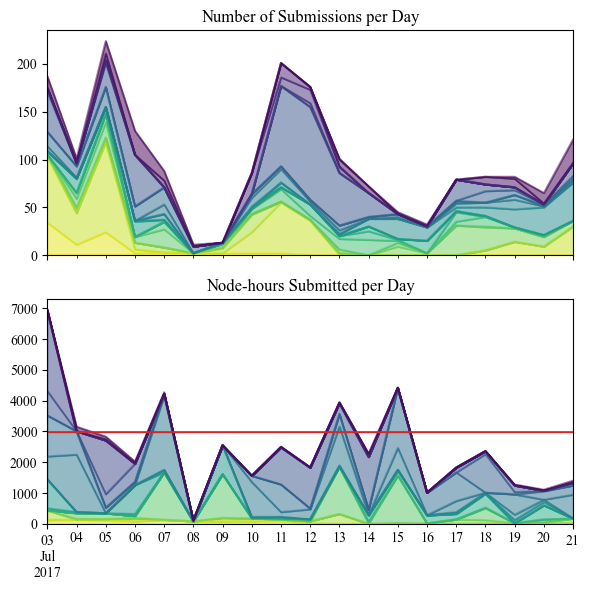
\includegraphics[clip,width=\linewidth,trim={0.1cm 8.3cm 0.1cm 0.75cm}]{figures/submissions.png}
    \caption{Number of submissions per day.}
    \label{fig:wl_distrib_sub_top}
\end{subfigure}

\vspace{1em} % Add vertical space between subfigures

% Bottom part of the figure
\begin{subfigure}[t]{0.8\linewidth}
    \centering
    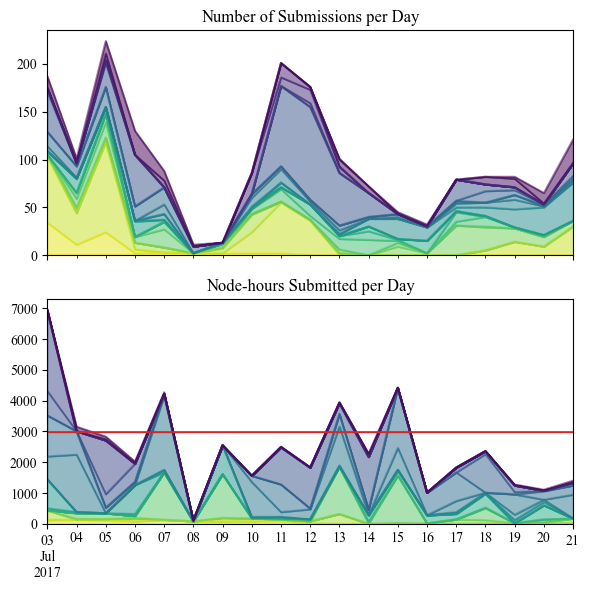
\includegraphics[clip,width=\linewidth,trim={0.1cm 1.1cm 0.1cm 7.5cm}]{figures/submissions.png}
    \caption{Node-hours submitted per day.}
    \label{fig:wl_distrib_sub_bottom}
\end{subfigure}

\caption{Distribution of job submissions and platform capacity over the days of July 2017 (x-axis).}
\label{fig:wl_distrib_sub}
\end{figure*}

\iffalse
\begin{figure*}[tbp]
\centering
    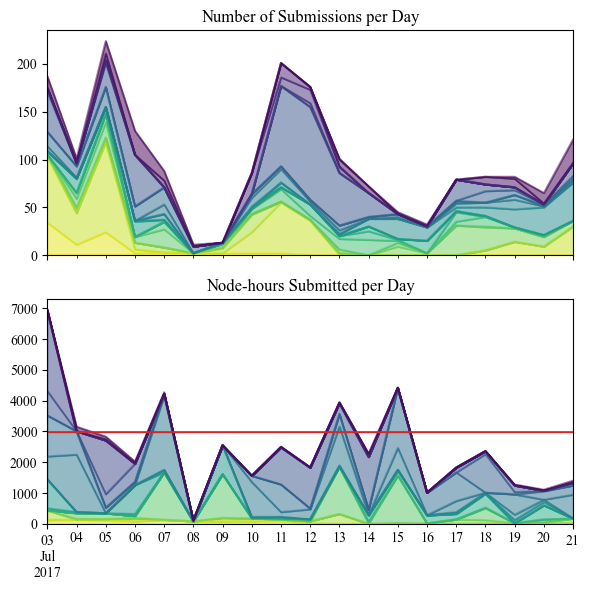
\includegraphics[clip,width=0.8\linewidth,trim={0.1cm 1.1cm 0.1cm 4.1cm}]{figures/submissions.png}
    \caption{Distribution of job submissions in the baseline workload over the days of July 2017 included in the period (X-axis). 
    \small
    Each color represents a different user.
    The horizontal line in the bottom graph is the maximum capacity of the platform
    ($M=124\times24=2,976$ node-hours per day).}
    \label{fig:wl_distrib_sub}
\end{figure*}
\begin{figure*}[tbp]
    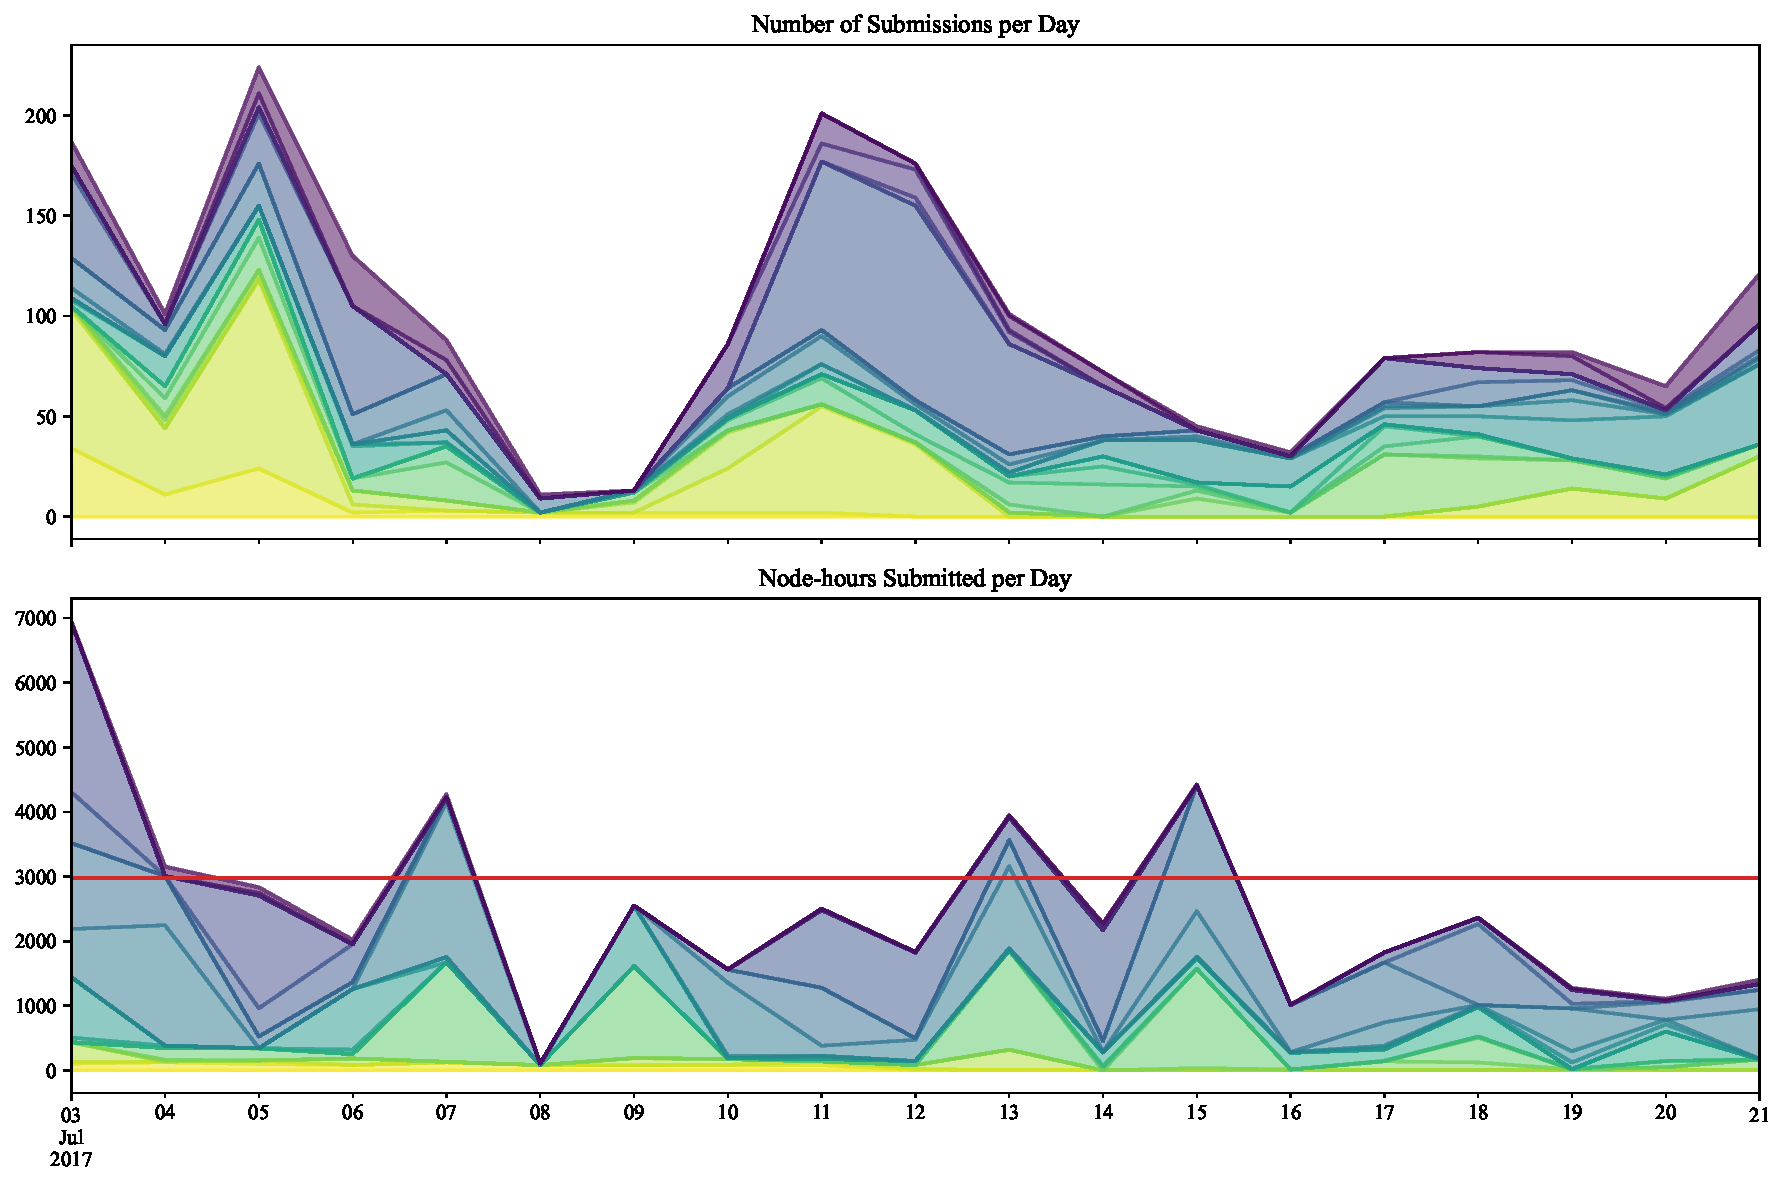
\includegraphics[clip,width=\linewidth,trim={0.1cm 0cm 0.1cm 0.1cm}]{figures/wl_user_sampling_july3-22.pdf}
    \caption{Distribution of job submissions in the baseline workload over the days of July 2017 included in the period (X-axis). 
    %\small
    Each color represents a different user.
    The horizontal line in the bottom graph is the maximum capacity of the platform
    ($M=124\times24=2,976$ node-hours per day).}
    \label{fig:wl_distrib_sub}
\end{figure*}
\fi

\begin{figure*}[tbp]
\centering
    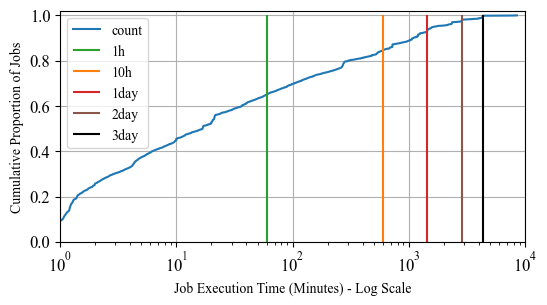
\includegraphics[clip,width=0.7\linewidth,trim={0.1cm 0.1cm 0.1cm 0.1cm}]{figures/distrib_job_size.png}
    \caption{Distribution of job execution time in the baseline workload.}
    \label{fig:wl_distrib_cum}
\end{figure*}

\begin{figure*}[tbp]
\centering

% Top part of the figure
\begin{subfigure}[t]{0.8\linewidth}
    \centering
    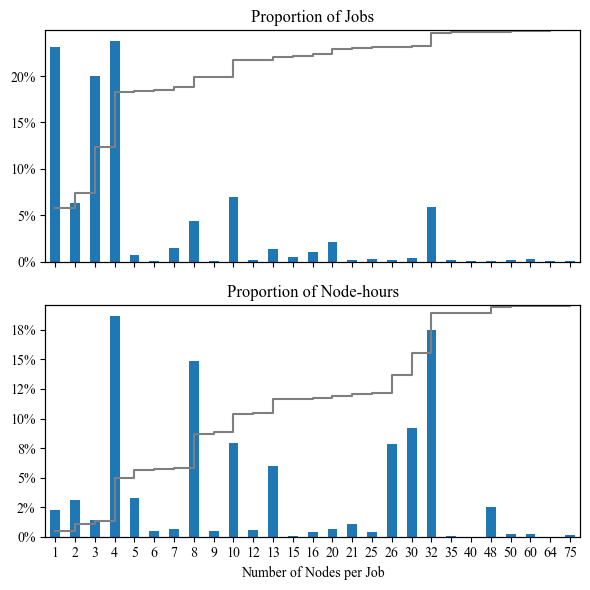
\includegraphics[clip,width=\linewidth,trim={0.1cm 8.1cm 0.1cm 0.75cm}]{figures/job_proportions.png}
    \caption{Proportion of jobs.}
    \label{fig:wl_distrib_runtime_size_top}
\end{subfigure}

\vspace{1em} % Add vertical space between subfigures

% Bottom part of the figure
\begin{subfigure}[t]{0.8\linewidth}
    \centering
    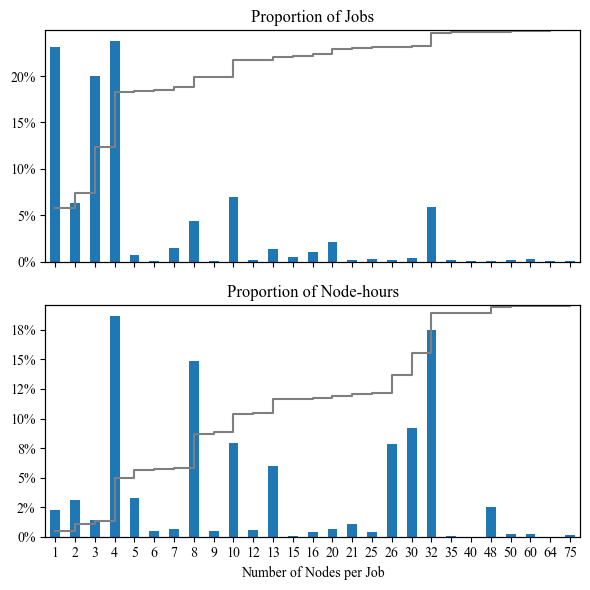
\includegraphics[clip,width=\linewidth,trim={0.1cm 0.1cm 0.1cm 7.75cm}]{figures/job_proportions.png}
    \caption{Proportion of node-hours.}
    \label{fig:wl_distrib_runtime_size_bottom}
\end{subfigure}

\caption{Job sizes in the baseline workload. The distribution is shown by the number of jobs (top) and number of node-hours (bottom), and the cumulative distribution is represented in grey.}
\label{fig:wl_distrib_runtime_size}
\end{figure*}

\iffalse
\begin{figure*}[tbp]
\centering
    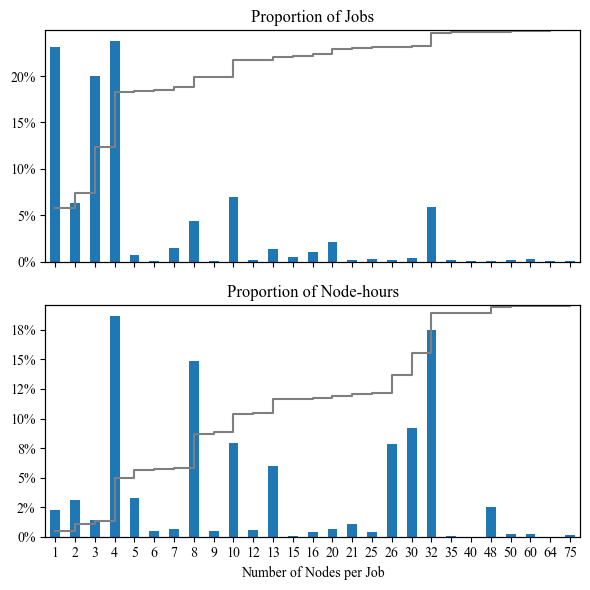
\includegraphics[clip,width=0.8\linewidth,trim={0.1cm 0.1cm 0.1cm 0.1cm}]{figures/job_proportions.png}
    \caption{Job size in the baseline workload.
    \small
    The distribution is shown by the number of jobs (top) and number of node-hours (bottom), and the cumulative distribution is represented in grey.}
    \label{fig:wl_distrib_runtime_size}
\end{figure*}
\begin{figure*}[tbp]
    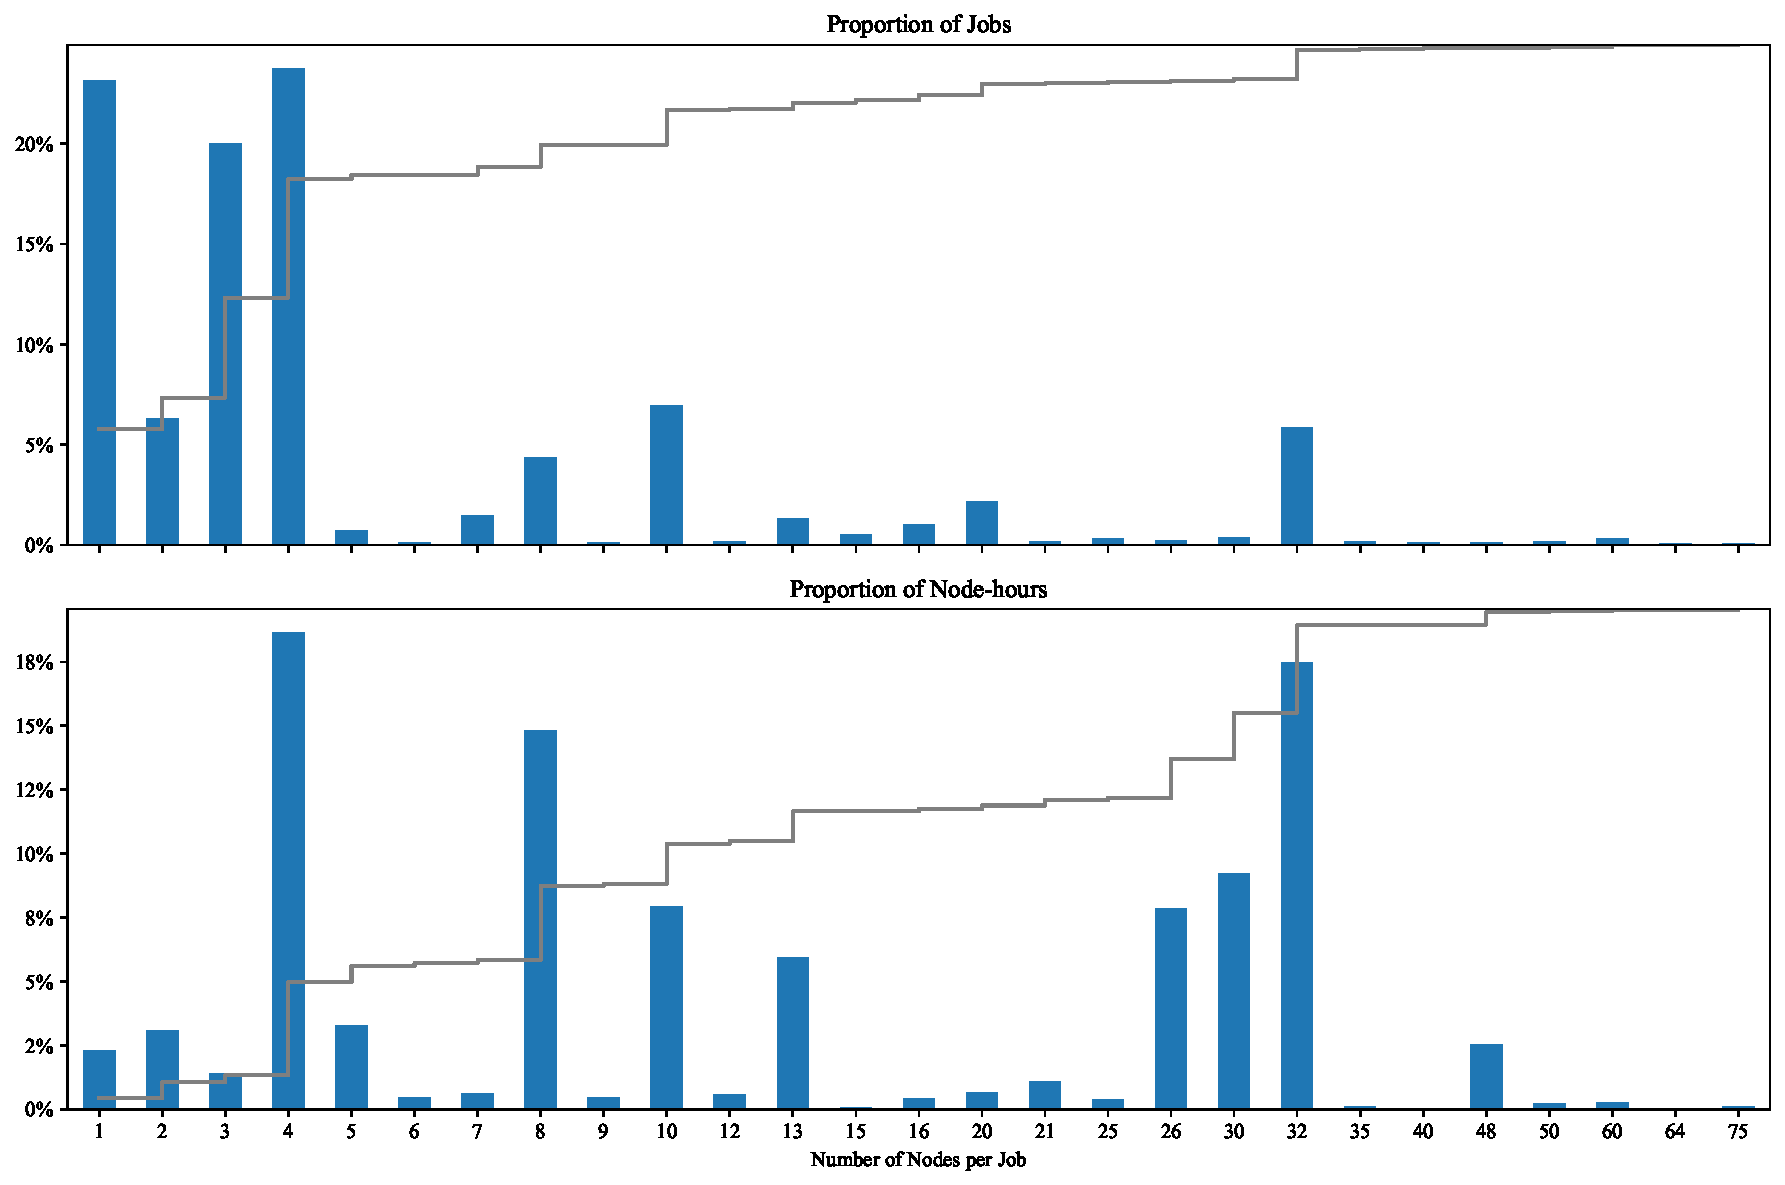
\includegraphics[clip,width=\linewidth,trim={0.1cm 0.1cm 0.1cm 0.1cm}]{figures/distrib_job_size_big_wl.pdf}
    \caption{Job size in the baseline workload.
    %\small
    The distribution is shown by the number of jobs (top) and number of node-hours (bottom), and the cumulative distribution is represented in grey.}
    \label{fig:wl_distrib_runtime_size}
\end{figure*}
\fi

\label{subsec:baseline}
The baseline workload is adapted from the most recent available workload
on the Parallel Workload Archive 
KIT-FH2-2016\footnote{\url{https://www.cs.huji.ac.il/labs/parallel/workload/l_kit_fh2/index.html}} log, recorded from the ForHLR II system located at the Karlsruhe Institute of Technology in Germany. 
Notice that this is the most recent workload publicly available and it is still a representative example of a general-purpose computational partition, unaffected by interference from deep learning jobs, better suited for accelerated partitions.
To adapt the log to our testbed, we perform the following steps:

\begin{enumerate}[wide]
    \item The original infrastructure has two queues: 
    the default queue with 1,152 20-core compute nodes, 
    and the visualization queue with 21 nodes comprising CPUs and GPUs.
    We focus on the first queue and exclude the GPU-enabled.

    \item The record is 1.5 years long, and we only have two days of computation available in our testbed. Consequently, we decide to speed up the replay by \textbf{applying a time-scaling factor of 10}, i.e., execution times and inter-arrival times are divided by 10 in the replay\footnote{This factor was chosen to balance the tradeoff between replaying more days from the original workload and suffering from overheads of phenomena that we cannot speed up (like the time taken by scheduling decisions).}.
    In this regard, we can replay $2\times10=20$ days from the original workload.

    \item 
    %\todo[inline]{SI@all: be careful with "burst" because that's not a limitation of our work and what does "good distribution" mean?} 
    By studying the distribution of job submissions over time,
    \mm{
    we select as representative the month of July 2017 because it features
    %is quite representative of the log:
    a homogeneous volume of submissions over days,
    well-distributed among users, and
    the presence of the characteristic day/night and weekday/weekend patterns.}
    %\st{no burst of submissions, presence of day/night and weekday/weekend patterns, and good distribution of submissions among the 68 users submitting in that period.}
    As a result, we select for the experiments \textbf{the 19-day period from July \nth{3} to July \nth{21} (included), 2017}.

    \item Finally, we \textbf{apply the user sampling method} described in Section~\ref{subsec:sampling}, 
    with a target in average node-hour per day of $.84M$, 
    where $M=124\times24$ is the maximum number of node-hour available per day in our testbed.
\end{enumerate}

The resulting workload contains 23 users \review{and 1,895 jobs}.
The median number of node-hours submitted per day is 2,272, i.e., 76\%  of the maximum capacity of the testbed.
The average number of node-hours submitted per day is 2,496, i.e., 84\% of the maximum capacity of the testbed.
Some characteristics of this workload are provided in the form of graphs.
Figure~\ref{fig:wl_distrib_sub} displays the number of daily submissions and node-hours submitted per day. 
Each color represents a particular user, and the stacked graphs show the submission volume per day.
Figure~\ref{fig:wl_distrib_cum} shows the cumulative proportion of jobs as a function of their duration. It shows that a vast majority lasts less than one hour (slightly more than 60\%).
Figure~\ref{fig:wl_distrib_runtime_size} shows the distribution of job execution times and job sizes. 
Jobs are mainly requesting 1, 3, or 4 nodes (see Figure~\ref{fig:wl_distrib_runtime_size_top}). 
But it also shows that large jobs (see 26, 30, and 32 nodes in the x-axis of Figure~\ref{fig:wl_distrib_runtime_size_bottom}), while rare, represent a significant part of the total executed mass.
Since the jobs in the log have a fixed duration, the replayed jobs submitted to the cluster will allocate resources for the same period, either by using \texttt{sleep} commands or implementing active waits.

\textbf{Warm-up Period.}
Looking at Figure~\ref{fig:wl_distrib_sub_bottom}, we note that the first day of the workload, July \nth{3}, features high activity in node-hours submitted.
This day, Monday, comes after a weekend of low activity on the platform. 
However, it is not until 11:00 AM that the platform runs in nominal conditions.
In other words, at that time, resources are virtually fully allocated, and there are pending jobs waiting for resources.
We thus define this period as a ``warm-up'' in the experiments, 
and malleable jobs start being submitted just after it ($t_0$ input of the \textit{generative user} described in Section~\ref{subsec:submitter}).

\subsection{A Generative User: The PhD Student}
\label{subsec:phdstudent}
To thoroughly evaluate our methodology, we count on \sergio{an additional generative user to submit jobs on top of the baseline workload.}
``The student'' is working with a simulation tool, particularly, a positive definite transport equation solver named MPDATA%
\footnote{
The MPDATA algorithm serves as the foundation of the EULAG multiscale fluid solver (Eulerian/semi-Lagrangian)~\cite{rojek_parallelization_2015}, which is responsible for calculating the advection of a non-diffusive quantity in a flow field.
}.
Its algorithm performs iterative time steps to simulate physical phenomena, requiring five input arrays and producing a single output array essential for subsequent time steps. 
The malleable version of MPDATA\footnote{Code available at \url{https://gitlab.bsc.es/siserte/mpdata-dmr}.} redistributes the input arrays between source and target processes, respectively, the number of processes before and after a reconfiguration.
MPDATA malleable demonstrated to increase the utilization of resources and reduce the power consumption in dynamic workloads~\cite{iserte_study_2020}.

For her study, the student must run ten instances ($N$) of MPDATA sequentially.
She will start launching jobs after the warm-up period and wait two scaled hours (720 actual seconds) before submitting the next job. 
This think time ($\Delta t$) corresponds to a hypothetical analysis of the results and the preparation of the subsequent execution.

The student is requested to complete her workload in 14 days; in other words, she has a deadline of two weeks to present her results.
Since she is in a hurry, an alarm is triggered on her phone when a job finishes, and she immediately starts processing data and setting up the next job.

MPDATA is configured with a computational domain of $8,192\times 1,024\times 128$ cells, iterating during 1,800 steps. 
This computational domain enables the user to run MPDATA from $1$ to $64$ nodes.
Figure~\ref{fig:mpdata-speedup} showcases the scalability of MPDATA with the given configuration in MN5.
The application scales up to $16$ nodes linearly, from where it shows speedups lower than $2x$.

\begin{figure*}[tbp]
    \centering
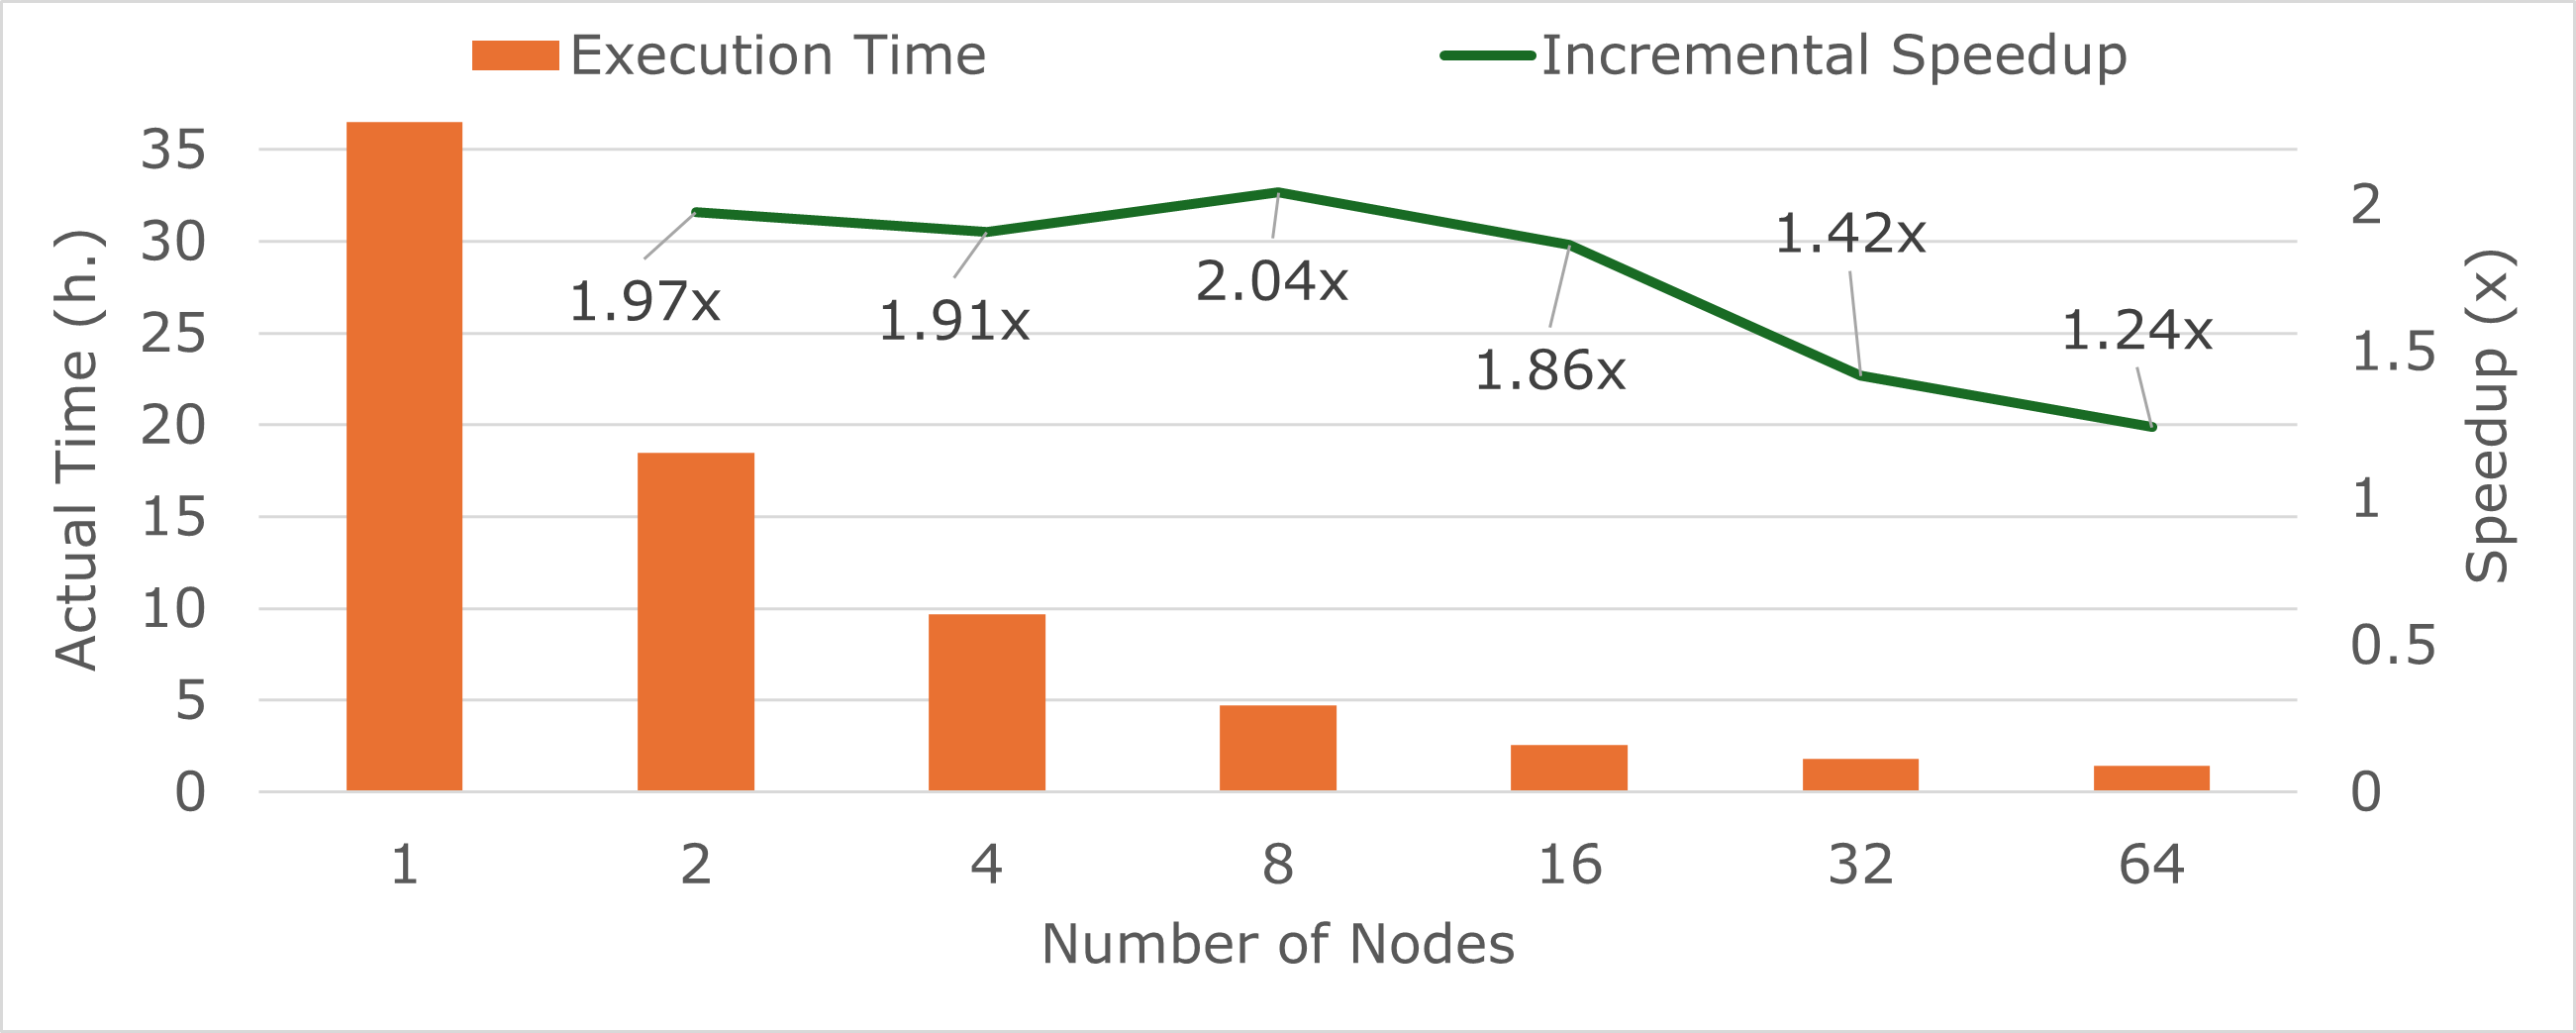
\includegraphics[clip,width=0.9\linewidth,trim={0.1cm 0.5cm 0.1cm 0.1cm}]{figures/mpdata.png}
    \caption{MPDATA scalability in MN5.}
    \label{fig:mpdata-speedup}
\end{figure*}

\begin{figure*}[tbp]
    \centering
    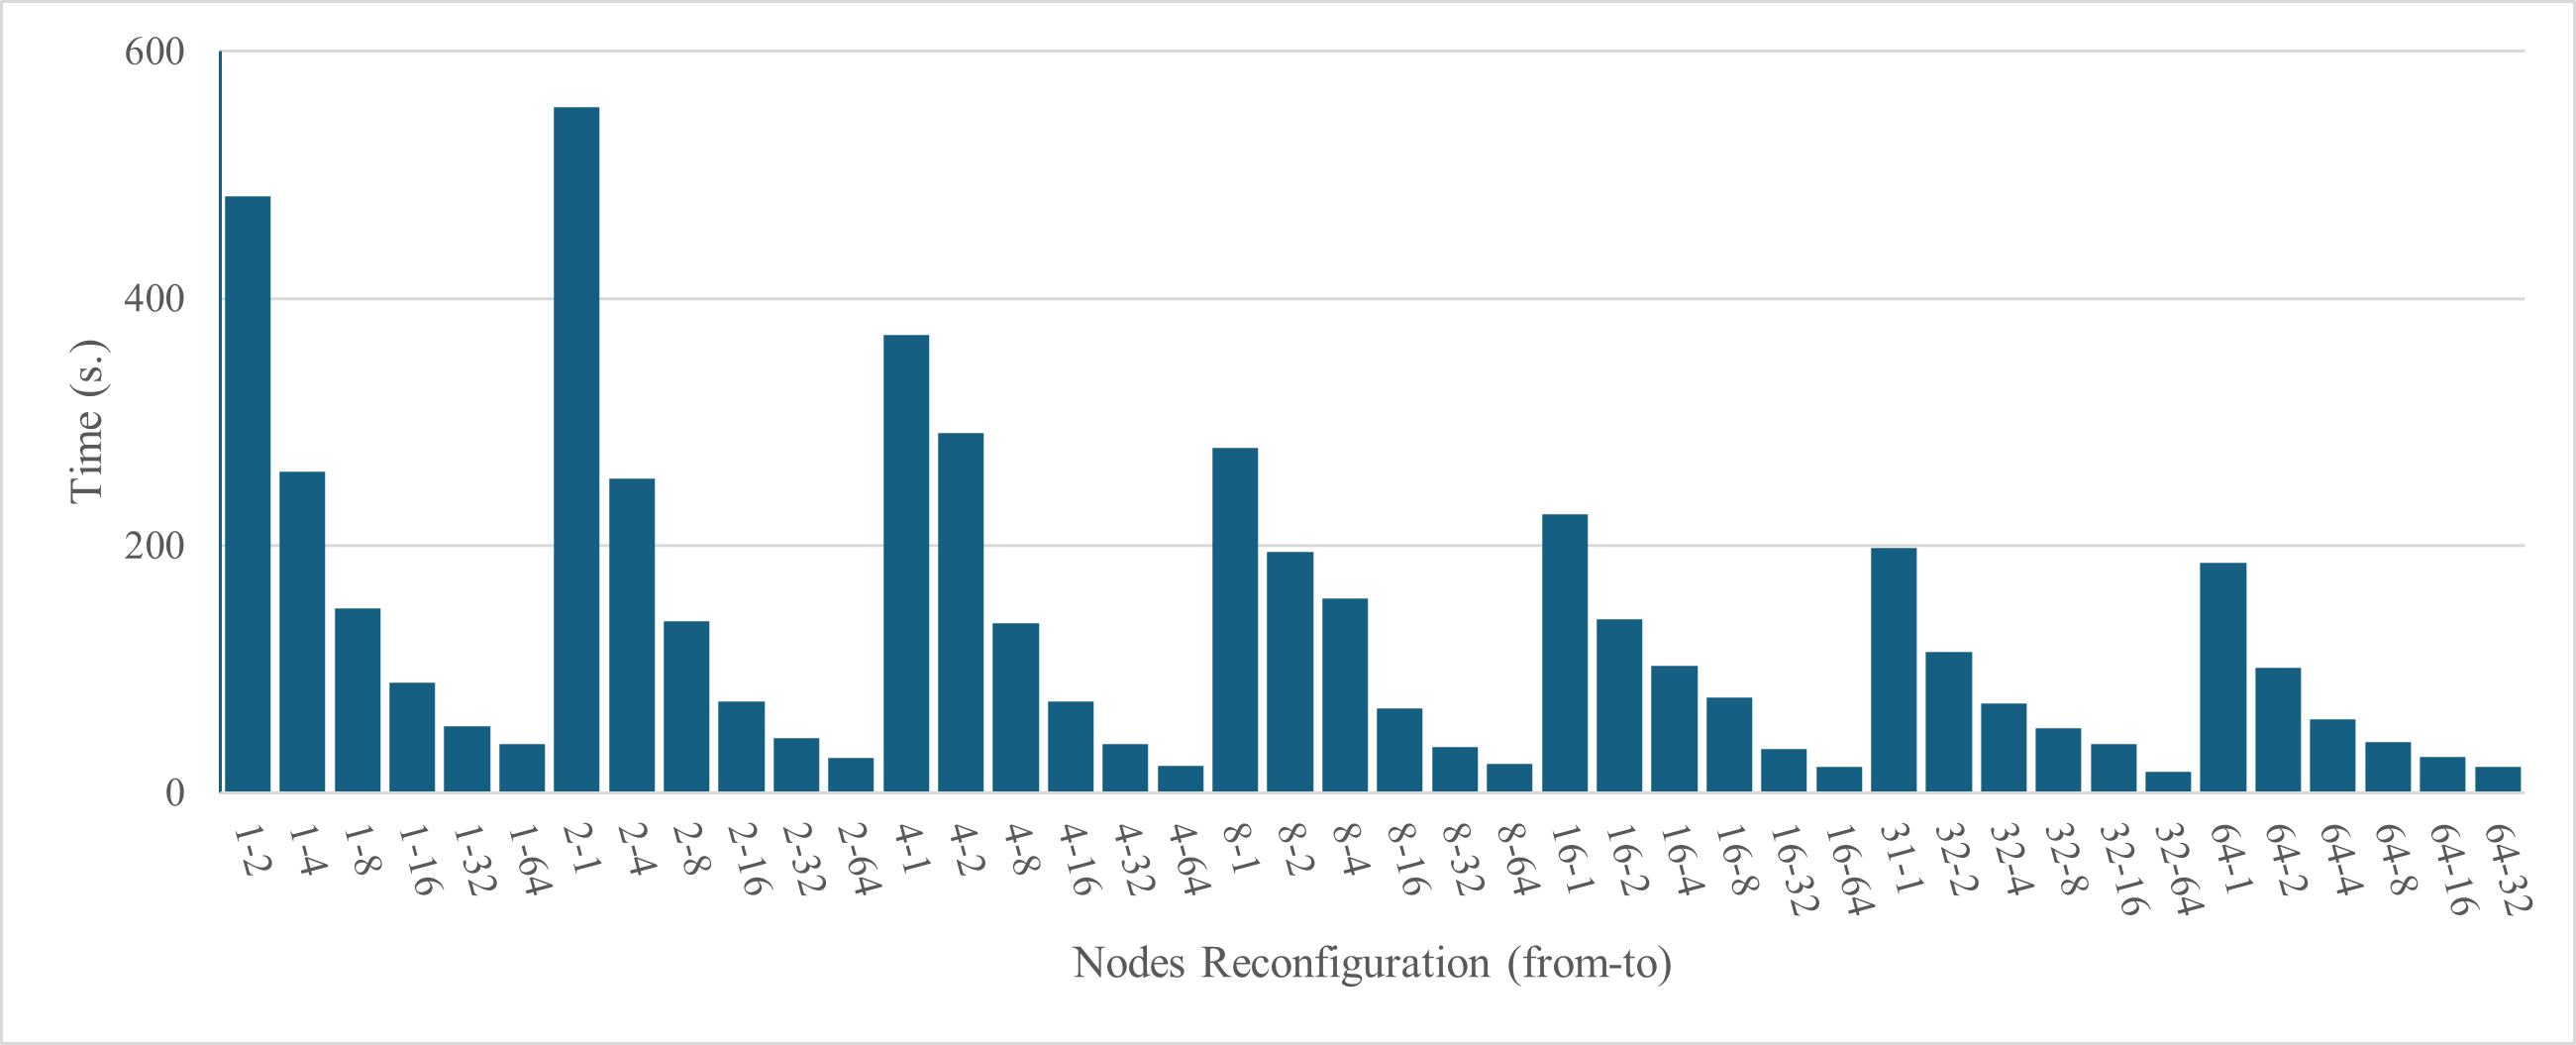
\includegraphics[clip,width=\linewidth,trim={0.5cm 0.25cm 0.1cm 0.2cm}]{figures/mpdata-reconf.png}
    \caption{MPDATA reconfiguration times in MN5.}
    \label{fig:mpdata-reconf}
\end{figure*}

\subsection{Experiments Definition}\label{subsubsec:exps}
Five experiments have been designed to study and analyze the effect of job malleability and dynamic management of resources over an existing workload.
\mm{Each experiment was launched on an independent 48-hour reservation of the 125-node testbed (see Section~\ref{subsec:testbed}).}
\begin{figure*}[tbp]
  \centering
  %\small
  \begin{minipage}{.6\linewidth}
    \begin{algorithm}[H]
    %\large
        \caption{Reconfiguration Policy Algorithm in Slurm}
        \label{alg:reconf_policy}
        \begin{algorithmic}[1]
            \STATE $\text{result} \gets \textsc{NONE}$
            \STATE $\eta \gets \textsc{EvaluateMyParallelEfficiency}()$
            \IF{$\textsc{JobCanBeInitiatedWithPartOfMyResources}()$}    
                \IF{$\eta < 0.85$}
                    \STATE $\textsc{SetMaximumPriorityToTargetPendingJob}()$
                     \STATE $\text{result} \gets \textsc{SHRINK}$
                \ENDIF
            \ELSE
                \STATE $\mathcal{R} \gets \textsc{ThereAreAvailableResources}()$
                \IF{$\mathcal{R} \neq \emptyset$}
                    \IF{$\eta > 0.10$}
                        \STATE $\text{result} \gets \textsc{EXPAND}$
                    \ENDIF
                \ENDIF
            \ENDIF
            \STATE \textbf{return} $\text{result}$
        \end{algorithmic}
    \end{algorithm}
  \end{minipage}
\end{figure*}
With these experiments, we will illustrate scenarios that represent different user behaviors:
\begin{enumerate}[wide]
    \item \textbf{Baseline}: this experiment corresponds to executing the baseline workload described in Section~\ref{subsec:baseline}. This experiment sets the original activity of the workload execution in the cluster.
    \item \textbf{StaticN32}: this experiment executes sequentially over the baseline workload, the 10-job workload of the PhD student launched with 32 nodes each.
    This is a realistic case, since with 32 nodes the execution time is $\approx14$ scaled hours (10x the actual time in Figure~\ref{fig:mpdata-speedup}). It means that she could finish her executions in less than six scaled days in an ideal scenario where jobs were not delayed.
    \item \textbf{StaticN16}: this is another non-malleable experiment similar to \textit{Static32} but launching the jobs with 16 nodes, instead.
    In this case, the student works with the shortest configuration time, the one within the 2x speedup in Figure~\ref{fig:mpdata-speedup}, which lasts $\approx18.5$ scaled hours.
    Theoretically, she could complete her executions in less than eight scaled days.
    We have discarded to configure a hypothetical \textit{Static8} experiment, since the theoretical time required to run the 10-job workload with eight nodes under ideal conditions is 47.5 scaled hours, while the maximum wall time granted for the experiment is 48 hours.
    \item \textbf{AlwaysGrow}: in this experiment, the PhD student instantiates malleable jobs over the baseline workload. Jobs are submitted moldable, requesting a 1--64 range of nodes. 
    Since she is under a tight deadline, she decides to disable shrinkages; jobs may only be expanded up to 64 nodes upon the RMS decision. By default, the reconfiguration policy will plan an expansion when sufficient resources are available to upscale.
    Furthermore, the student has defined a reconfiguration inhibitor of \texttt{\#current\_nodes} iterations to avoid abuse of reconfiguration operations and reduce overhead generated by them (see Figure~\ref{fig:mpdata-reconf}).
    \item \textbf{ParEfficiency}: in this case, jobs are submitted within the 2--64 nodes range.
    Malleability limits are defined as one node at the minimum and 64 at the maximum.
    However, the student configures an additional inhibitor for reconfigurations longer than 50 scaled minutes. 
    According to Figure~\ref{fig:mpdata-reconf}, which depicts the measured reconfiguration time for all the possible node combinations of \textit{from--to} reconfigurations, those greater than five minutes are avoided, specifically the reconfigurations \textit{1 to 2}, \textit{2 to 1}, and \textit{4 to 1}.
    This experiment leverages the performance-aware support of the dynamic resource manager (see Section~\ref{subsec:dmr}). 
    Algorithm~\ref{alg:reconf_policy} depicts the reconfiguration policy.
    Every time a malleable job triggers a reconfiguration, Slurm will determine the action that the DMRlib runtime must perform.
    In this regard, Slurm's plugin will check if a pending job may be initiated with some of the resources that would be available if the malleable job relinquishes them after its shrinkage (line~3).
    If a target job may be initiated, the policy checks the current parallel efficiency of the malleable job.
    If the parallel efficiency does not reach a minimum threshold (line~4), the target job priority in the queue will be increased (line~5), and the malleable job will be shrunk (line~6).
    If no job may be initiated and there are available resources in the cluster (line~10), the policy checks the current parallel efficiency. If the value exceeds a determined threshold (line~11), indicating that the execution may still leverage additional resources, the malleable job will be expanded (line~12).

    This policy aims to obtain as many resources as possible if no other job in the queue may use them. However, suppose any job in the queue may be initiated, and the malleable job is not reasonably using the resources (within a parallel efficiency threshold). In that case, the RMS reassigns the resources to a pending job in order to increase global cluster productivity and efficiency.
\end{enumerate}

%%%%%%%%%%%%%%%%%%%%%%%%%%%%%
\section{Results}
\label{sec:results}
In this section, the results obtained after running the experiments are analyzed.
We use the following metrics for the validation of MPI malleability: makespan (Section~\ref{subsec:makespan}), resource allocation rate (Section~\ref{subsec:utilization}), and waiting time (Section~\ref{subsec:wt})%
\footnote{
Since the execution time is fixed and determined by the log, and the completion time is the sum of waiting plus execution times, the completion time is entirely dependent on the waiting time.
}.

Note that the metrics have different interpretations depending on the type of workload replay, as well-explained by Feitelson~\cite{feitelson_resampling_2021}.
In the case of replay with feedback (like here with the PhD student workload), the primary performance metric is the makespan, i.e., the total time to execute the workload.
On the contrary, the makespan in timestamp-based replay (like here with the baseline workload) is dictated by the original submission timestamps.
In this case, the primary performance metric is the waiting times for each job.

\begin{table*}[tbp]
    \fontsize{9.5pt}{20pt}\selectfont
    \centering
    \begin{tabular}{lcccccc}
        \toprule
         & & \textbf{Baseline} & \textbf{StaticN32} & \textbf{StaticN16} & \textbf{AlwaysGrow} & \textbf{ParEfficiency} \\
        \midrule
        \multirow{2}{*}{\textbf{Workload Maskespan}} 
            & \textbf{Complete}     & 44.84 h.      & 45.15 h.   & 44.84 h.   & 44.84 h.   & 44.84 h. \\
            & \textbf{Only PhD}     & -             & 45.15 h.   & 38.50 h.   & 36.62 h.   & 32.88 h. \\
        \midrule
        \multirow{2}{*}{\textbf{Global Resource Allocation}} 
            & \textbf{Avg}     & 83.70\%     & 93.86\%   & 91.50\%   & 92.63\%   & 91.86\% \\
            & \textbf{Std}    & 24.07\%     & 11.44\%   & 17.62\%   & 17.24\%   & 17.16\% \\
        \midrule
        \multirow{2}{*}{\textbf{Actual Jobs Waiting Time}}
            & \textbf{Avg}     & 1,725.04 s.    & 3,007.24 s.     & 3,290.38 s.    & 4,365.89 s.     & 4,242.71 s.         \\
            & \textbf{Std}     & 4,450.38 s.    & 6,197.19  s.    & 7,677.89 s.    & 10,013.08 s.    & 11,690.31 s.        \\
        \bottomrule
    \end{tabular}
    \caption{Workloads makespan and average and standard deviation of allocated resources and waiting time for the five experiments, excluding the warm-up period.}
    \label{tab:alloc-wait}
\end{table*}


\begin{figure*}[tbp]
\centering
    \begin{overpic}[clip, width=0.95\linewidth, trim={0.1cm 0.1cm 0.1cm 0.2cm}]{figures/Baseline.png}
        \put(73.95,4){\color{gray}\line(0,1){33}}
        \put(75,10){\color{gray}\small Deadline}
    \end{overpic}
    \caption{Resource allocation (Y-axis) in each second of the execution (X-axis) for the \textit{Baseline} experiment.}
    \label{fig:baseline}
\end{figure*}

\subsection{Makespan}\label{subsec:makespan}
\review{
The completion time of the workload, or workload makespan, is a critical metric for the PhD student, who has a deadline to meet.
Particularly, she needs to focus on the time it takes to complete her 10-job workload.
Table~\ref{tab:alloc-wait} compiles execution metrics of the different experiments.
The first two rows of Table~\ref{tab:alloc-wait} (after the header) report the execution times for the two workloads. The first row corresponds to the complete workload (Baseline + PhD student), which also defines the overall experiment duration, while the second row refers exclusively to the PhD student workload.
\\\indent
As discussed in the introduction of this section, the first row is not meaningful, since makespan is dictated by the rigid submission timestamps replayed from the original log.
This is why all the values in this row are equal to the \textit{Baseline} makespan.
The only exception is \textit{StaticN32}, whose makespan is ruled by the PhD job, as shown in Figure~\ref{multifig:static32}.
The difficulty of scheduling large jobs in a congested system is manisfested in this experiment that reportes a completion time increased compared to \textit{Baseline}.
\\\indent
In the remaining experiments (\textit{StaticN16}, \textit{AlwaysGrow}, and \textit{ParEfficiency}), the PhD student jobs are completed before the end of the baseline workflow.
Of course, reducing the PhD student jobs size from 32 to 16 nodes helps the backfilling scheduler to find gaps to fit the jobs, thus reducing the PhD student workload completion time from 45.15 to 38.50 actual hours.
However, it is not enough to meet the student's deadline of 14 scaled days.
Figure~\ref{multifig:static16} shows that the last two jobs of the student are still running after the deadline.
\textit{AlwaysGrow}, leverages malleability to reduce the student makespan, but it still needs 36.62 actual hours, which is still beyond the deadline (see Figure~\ref{multifig:dyngrow}).
Notably, the ``smartest'' dynamic configuration, \textit{ParEfficiency}, needs $\approx73\%$ the time to complete the student jobs compared to \textit{StaticN32} (32.88 h. vs 45.15 h., respectively) without delaying the baseline workload and meeting the deadline, since both full workloads are completed in 44.84 h.
To sum up, Figure~\ref{multifig:dynpe} shows that the last job of the student finishes before the deadline in \textit{ParEfficiency} scenario.
\\\indent
In the following subsections, we will see how malleability affects the resource allocation rate and the waiting time, which are the two factors that explain the makespan reduction of the PhD student workload.
}

\begin{figure*}[tbp]
    \centering

    \begin{subfigure}[t]{0.95\textwidth}
        \centering
        \begin{overpic}[clip, width=\linewidth, trim={0.1cm 1.4cm 0.1cm 0.2cm}]{figures/StaticN32.png}
            \put(73.5,0){\color{gray}\line(0,1){32}}
            \put(74.55,10){\color{gray}\small Deadline}
        \end{overpic}
        \caption{\textit{StaticN32}}
        \label{multifig:static32}
        \vspace{3mm}
    \end{subfigure}

    \begin{subfigure}[t]{0.95\textwidth}
        \centering
        \begin{overpic}[clip, width=\linewidth, trim={0.1cm 0.1cm 0.1cm 0cm}]{figures/StaticN16.png}
            \put(73.95,4){\color{gray}\line(0,1){33}}
            \put(75,10){\color{gray}\small Deadline}
        \end{overpic}

        \caption{\textit{StaticN16}}
        \label{multifig:static16}
    \end{subfigure}

    \caption{
    Resource allocation (Y-axis) over execution time (X-axis) for the \textit{student} \texttt{static} experiments. 32-node allocations are harder to fit, increasing makespan.}
    \label{fig:static-experiments}
\end{figure*}

\begin{figure*}[tbp]
    \centering

    \begin{subfigure}[t]{0.95\textwidth}
        \centering
        \begin{overpic}[clip, width=\linewidth, trim={0.1cm 1.4cm 0.1cm 0.2cm}]{figures/AlwaysGrow.png}
            \put(73.95,0){\color{gray}\line(0,1){32}}
            \put(75,10){\color{gray}\small Deadline}
        \end{overpic}

        \caption{\textit{AlwaysGrow}}
        \label{multifig:dyngrow}
        \vspace{3mm}
    \end{subfigure}

    \begin{subfigure}[t]{0.95\textwidth}
        \centering
        \begin{overpic}[clip, width=\linewidth, trim={0.1cm 0.1cm 0.1cm 0cm}]{figures/ParEfficiency.png}
            \put(73.95,4){\color{gray}\line(0,1){33}}
            \put(75,10){\color{gray}\small Deadline}
        \end{overpic}
        
        \caption{\textit{ParEfficiency}}
        \label{multifig:dynpe}
    \end{subfigure}

    \caption{
    Resource allocation (Y-axis) over execution time (X-axis) for the \textit{student} \texttt{dynamic} experiments. Dynamic policies, especially \textit{ParEfficiency}, reduce makespan.}
    \label{fig:dynamic-experiments}
\end{figure*}

\iffalse
\begin{figure*}[tbp]
    \centering
    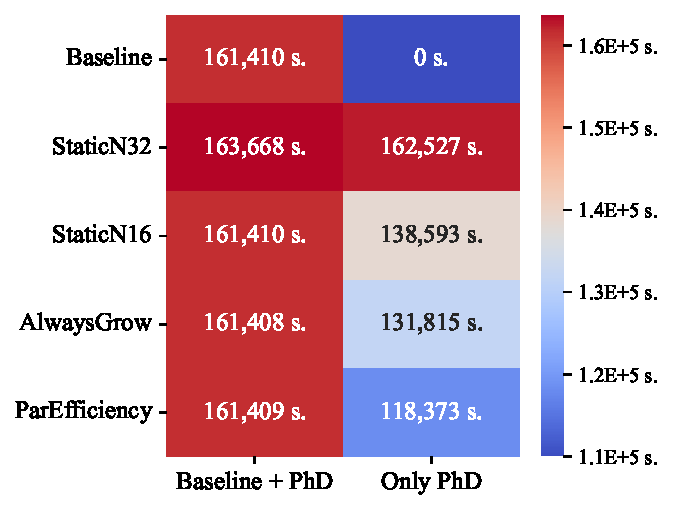
\includegraphics[clip,width=0.6\linewidth,trim={0.1cm 0.1cm 0.1cm 0.1cm}]{figures/heatmap.pdf}
    \caption{Heatmap representing the makespan (s.) of experiments (Y-axis) and workloads (X-axis). \textit{ParEfficiency} completes the \textit{student} workload in 73\% of the \textit{StaticN32} time.}
    \label{fig:heatmap}
\end{figure*}
\fi

\subsection{Resource Allocation Rate}\label{subsec:utilization}
Figure~\ref{fig:baseline} showcases the total number of allocated nodes for every actual second of the \textit{Baseline} experiment.
Correspondingly, figures~\ref{multifig:static32},~\ref{multifig:static16},~\ref{multifig:dyngrow}, and~\ref{multifig:dynpe} showcase stacked bar plots where each timestamp depicts the sum of the allocated resources by the baseline plus the PhD student workloads.
The figures present different patterns: while the static experiments in figures~\ref{multifig:static32} and~\ref{multifig:static16} show how the student jobs have to wait for slots that satisfy the static requests, the malleable experiments in figures~\ref{multifig:dyngrow} and~\ref{multifig:dynpe} leverage fragmentation where student jobs run.

\review{
Table~\ref{tab:alloc-wait} contains in the \nth{4} row the allocation rate for each experiment, which is the average node utilization over the makespan of the experiment, excluding the warm-up period.
In turn, the \nth{5} row presents the standard deviation of the allocation rate.
\\\indent
\textit{Baseline} provides the lower average allocation rate with the highest standard deviation, which is expected since the platform presents many idle regions of resources during the execution (see Figure~\ref{fig:baseline}).
Evidently, the remaining experiments present higher allocation rates because of the 10 extra jobs of the PhD student.
While \textit{StaticN32} presents the highest average allocation rate, it also shows the lowest standard deviation, which means that the platform is uniformly more saturated during the experiment (see Figure~\ref{multifig:static32}).
The remaining experiments present similar average allocation rates, with higher standard deviations than \textit{StaticN32}, which means that the platform presents more idle regions during the execution (see figures~\ref{multifig:static16},~\ref{multifig:dyngrow}, and~\ref{multifig:dynpe}), particularly at the end of the workload execution, when the jobs of the baseline workload are still running, but the PhD student jobs have already finished.
In this regard, the rigid jobs of \textit{StaticN16} and the malleable jobs of \textit{AlwaysGrow} and \textit{ParEfficiency} make no difference in the allocation rate.
That is why we need to understand better the makespan reduction of the PhD student workload with studying the waiting time in the next section, where we see how MPI malleability can maintain resource utilization while reducing the completion times.
}

\subsection{Waiting time}\label{subsec:wt}
\review{
To analyze how baseline jobs are affected by the submission of jobs from the PhD student, we look at their average waiting times and standard deviation in the different scenarios (see Table~\ref{tab:alloc-wait}, \nth{6} and \nth{7} rows).
\\\indent
It is patent that the original workload suffers longer delays on average when the PhD student jobs are submitted: the average waiting time increases from 1,725.04 s. to 3,007.24 s. or 4,365.89 s. in the best and worst cases, respectively.
This increment of up to $\approx2.53x$ is expected since the system is more saturated with the extra jobs.
\\\indent
Besides, the two dynamic experiments (\textit{AlwaysGrow} and \textit{ParEfficiency}) pose a larger impact on the baseline waiting time, in terms of average and standard deviation.
This can be explained by the greedy nature of the malleable configurations, starting with fewer resources and expanding as resources are released in the platform, making the baseline jobs wait longer.
}

\iffalse
\begin{figure*}[tbp]
    \centering
    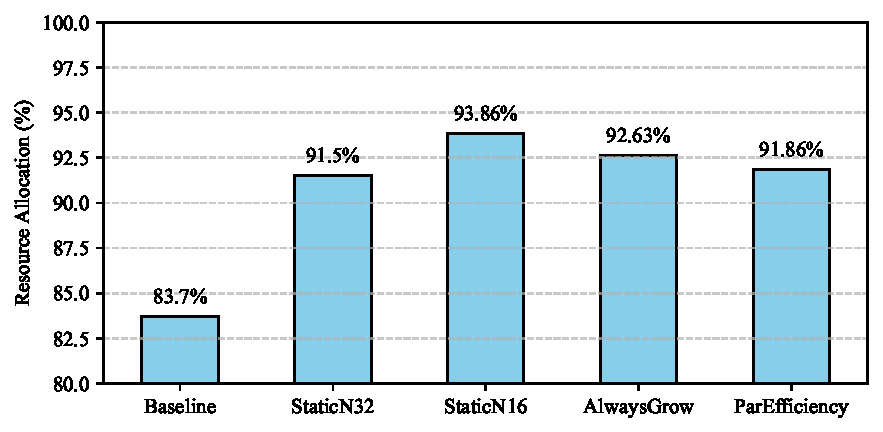
\includegraphics[clip,width=0.75\linewidth,trim={0.1cm 0.1cm 0.1cm 0.1cm}]{figures/resourceAlloc.pdf}
            \caption{Average percentage of allocated resources (Y-axis) for the five experiments (X-axis). \textit{ParEfficiency} has a more balanced resource allocation rate while reducing the makespan.}
    \label{fig:resource_allocation}
\end{figure*}

\begin{figure*}[tbp]
        \centering
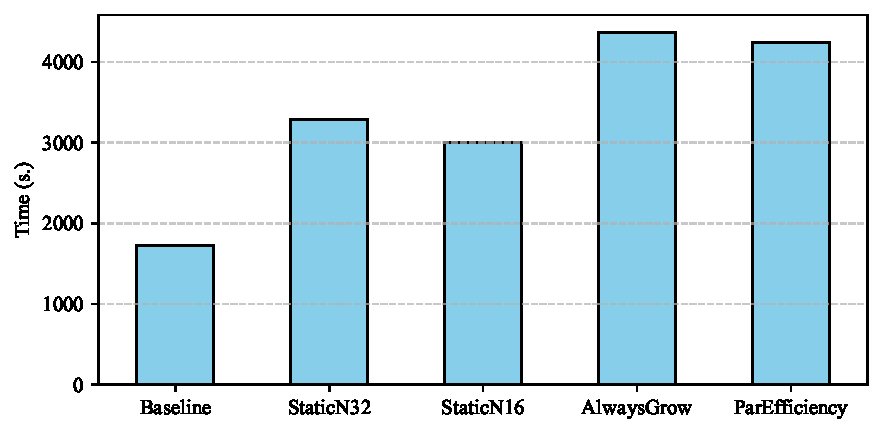
\includegraphics[clip,width=0.75\linewidth,trim={0.1cm 0.1cm 0.1cm 0.1cm}]{figures/base-waiting.pdf}
        \caption{Average waiting time of the baseline jobs (Y-axis) for the five experiments (X-axis). \texttt{Dynamic} experiments need more time to fit queued jobs in favor of the makespan.}
        \label{fig:baseline_waiting}
\end{figure*}
\fi

In a finer detailed analysis, we studied the accumulated waiting time throughout the execution (Figure~\ref{fig:waitAcc}).
It shows how the waiting time increases as new jobs arrive in the queue, and since there are not enough available resources until around timestamp 77,000 (July \nth{10}), they cannot be quickly started.
After this milestone, the waiting time progressively starts growing again. 
More specifically, Figure~\ref{fig:waitDiff} showcases the waiting time difference of the various experiments compared to the Baseline for each job.
One of the most valuable insights we extract is the behavior detected around job $750$ (July \nth{10}), where waiting times drop.
This is because there is a period around July \nth{8} and \nth{9}, as shown in Figure~\ref{fig:wl_distrib_sub_top}, where the submissions drastically decrease, and it takes over a day to drain the queue.
That is why jobs submitted after that event present a virtually null waiting time.

\begin{figure*}[tbp]
    \centering
    \begin{overpic}[clip,width=0.95\linewidth,trim={0.1cm 0.1cm 0.1cm 0.1cm}]{figures/waitAcc.png}
        % Draw a vertical line at the desired X position (percentage of width)
        \put(48.4,4){\color{gray}\line(0,1){26}} % Vertical line
        % Add text next to the line (adjust 52 and 50 for position)
        \put(49.5,18){\color{gray}\small July \nth{10}} % Text next to the line
    \end{overpic}
    \caption{Accumulated waiting time throughout the workloads executions.}% The red line points out a change in the submission rate.}
    \label{fig:waitAcc}
\end{figure*}

\begin{figure*}[tbp]
    \centering
    \begin{overpic}[clip,width=0.95\linewidth,trim={0.1cm 0.1cm 0.1cm 0.1cm}]{figures/waitDiff.png}
        % Draw a vertical line at the desired X position (percentage of width)
        \put(44.8,4){\color{gray}\line(0,1){29}} % Vertical line
        % Add text next to the line (adjust 52 and 50 for position)
        \put(45.8,24){\color{gray}\small July \nth{10}} % Text next to the line
    \end{overpic}
    \caption{Difference in job waiting times compared to the baseline experiment.} %The red line points out a change in the submission rate.}
    \label{fig:waitDiff}
\end{figure*}

\subsection{Focus on the PhD Student}
Figure~\ref{fig:phd_completion} illustrates the average completion time of the student's jobs.
The completion time is composed of the sum of the waiting time and the execution time. 
The malleable experiments present a higher execution time compared to their static counterpart.
\review{
This is because malleable jobs are likely to be initiated with fewer resources, because they are submitted with a range of nodes, and the RMS will assign them the minimum available resources at that time benefiting from backfilling.
For this reason, \textit{Student}'s jobs barely wait in the with malleability.
}

Then, malleable jobs are progressively expanded following their respective reconfiguration policies.
The more resources assigned to the jobs, the lower the execution time (see Figure~\ref{fig:mpdata-speedup}). 
However, reconfigurations come with a cost (see Figure~\ref{fig:mpdata-reconf}), and this cost is included in the execution time.

\begin{figure*}[tbp]
    \centering
        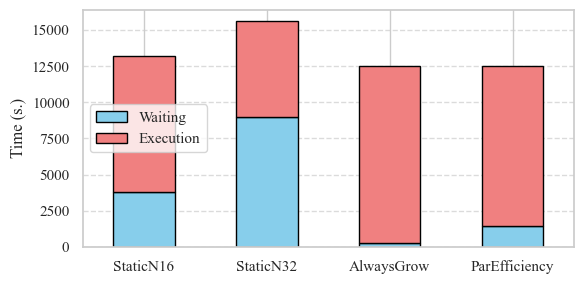
\includegraphics[clip,width=0.95\linewidth,trim={0.1cm 0.1cm 0.1cm 0.1cm}]{figures/phd-stacked.png}
        \caption{Average student's job completion (waiting + execution) time (Y-axis) for the four experiments (X-axis).}
        \label{fig:phd_completion}
\end{figure*}

\begin{figure*}[tbp]
    \centering
        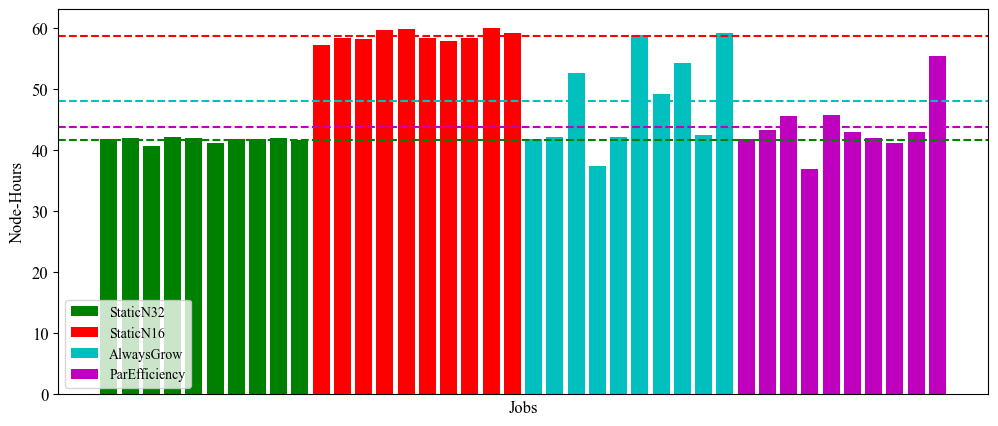
\includegraphics[clip,width=0.95\linewidth,trim={0.2cm 0.1cm 0.2cm 0.1cm}]{figures/node-hours3.png}
        \caption{Individual student job's Node-hours (Y-axis) grouped by colors for the four experiments (X-axis). Dashed lines represent the average per experiment (Y-axis).}
        \label{fig:phd_nodehours}
\end{figure*}

\review{
The total cost of reconfigurations in our case is given in Table~\ref{tab:reconfig}.
Additionally, Table~\ref{tab:reconfig_pairs} details the reconfigurations performed in the \textit{ParEfficiency} experiment.
}

\iffalse
\begin{table*}[tbp]
\centering
\fontsize{9.5}{14pt}\selectfont
\begin{tabular}{lccc}
\toprule
 & \textbf{\#} & \textbf{Mean Time} & \textbf{Overhead} \\
\midrule
AlwaysGrow & 27+0 & 160 s. & 4,332 s. \\
ParEfficiency & 18+7 & 77 s. & 1,929 s. \\
\bottomrule
\end{tabular}
\caption{Per experiment (first column) we find the number of reconfigurations in format \textit{expansions + shrinkages} (second column), reconfiguration mean time (third column), and reconfiguration overhead (fourth column).
}
\label{tab:reconfig}
\end{table*}
\fi

\begin{table*}[tbp]
\centering
\fontsize{9.5pt}{14pt}\selectfont
\begin{tabular}{l r r r  r r r  r r r}
    \toprule
    & \multicolumn{3}{c}{Expansions} & \multicolumn{3}{c}{Shrinkages} & \multicolumn{3}{c}{Total} \\
    \cmidrule(lr){2-4} \cmidrule(lr){5-7} \cmidrule(lr){8-10}
    & \# & Avg. & Overhead & \# & Avg. & Overhead & \# & Avg. & Overhead \\
    \midrule
    AlwaysGrow   & 27 & 160 s. & 4,332 s. & 0  & --    & 0 s.    & 27 & 160 s. & 4,332 s. \\
    ParEfficiency & 18 &  87.8 s.  & 1,580 s. & 7  & 48.9 s. &  349 s.  & 25 & 76.9 s.  & 1,929 s. \\
    \bottomrule
\end{tabular}
\caption{Per experiment: number of reconfigurations (expansions / shrinkages), average reconfiguration time and accumulated overhead (actual seconds).}
\label{tab:reconfig}
\end{table*}

In \textit{ParEfficiency}, the overhead is reduced thanks to preventing the slowest reconfigurations.
Furthermore, since the malleable jobs are adapted to the workload and the performance, there are seven \textit{32 to 16}-node shrinkages to increase productivity by reducing the student workload time by 10\% compared to \textit{AlwaysGrow}.

If we pay attention to the node-hours consumed by the PhD Student jobs, Figure~\ref{fig:phd_nodehours} shows that metric for each of those jobs in the experiments. 
Furthermore, a dashed line represents the PhD student jobs mean node-hour per experiment.

Static jobs present a virtually constant node-hour consumption (standard deviation $<$ $1$). 
As shown in Figure~\ref{fig:mpdata-speedup}, the PhD jobs deliver lower speedup running on 32 than in 16 nodes, $1.41x$ and $1.86x$, respectively.
For this reason, the consumption is 17 node-hours higher in the \textit{StaticN32} experiment.
Regarding MPI malleability, since those jobs can be resized, they show variable node hours within the experiments (standard deviation $>$ $4$).
Remarkably, \textit{AlwaysGrow} and \textit{ParEfficiency} contain the two ``cheapest'' jobs because they run most, or the whole of their time, respectively, in 8 nodes. It is with eight nodes that the maximum performance is attained.

\begin{table}
\caption{Reconfigurations in the \textit{ParEfficiency} experiment (time in actual seconds). Gray rows represent shrinkages.}
\label{tab:reconfig_pairs}
\begin{tabular}{clll}
\toprule
\textbf{PhD Job Id}& \textbf{Initial Nodes} & \textbf{Final Nodes} & \textbf{Rec. Time} \\
\midrule
 \multirow{1}{*}{\textbf{0}} 
            & 16 & -- & -- \\
\midrule
 \multirow{3}{*}{\textbf{1}} 
            & 2 & 4 & 254 s. \\
            & 4 & 8 & 136 s.\\
            & 8 & 16 & 72 s.\\
\midrule
 \multirow{4}{*}{\textbf{2}} 
            & 8 & 16 & 69 s.\\
            & 16 & 32 & 43 s.\\
            & \cellcolor{lightgray}32 & \cellcolor{lightgray}16 & \cellcolor{lightgray}47 s.\\
            & 16 & 32 & 34 s.\\
\midrule
 \multirow{1}{*}{\textbf{3}} 
            & 8 & -- & -- \\
\midrule
 \multirow{4}{*}{\textbf{4}} 
            & 4 & 8 & 133 s.\\
            & 8 & 16 & 69 s.\\
            & 16 & 32 & 35 s.\\
            & \cellcolor{lightgray}32 & \cellcolor{lightgray}16 & \cellcolor{lightgray}49 s.\\
\midrule
 \multirow{1}{*}{\textbf{5}} 
            & 8 & 16 & 68 s.\\
\midrule
\multirow{1}{*}{\textbf{6}} 
            & 8 & 16 & 66 s.\\
\midrule
\multirow{1}{*}{\textbf{7}} 
            & \cellcolor{lightgray}32 & \cellcolor{lightgray}16 & \cellcolor{lightgray}47 s.\\
\midrule
\multirow{3}{*}{\textbf{8}} 
                & 2 & 4 & 253 s.\\
                & 4 & 8 & 135 s.\\
                & 8 & 16 & 67 s.\\
\midrule
 \multirow{8}{*}{\textbf{9}} 
            & 16 & 32 & 38 s.\\
            & \cellcolor{lightgray}32 & \cellcolor{lightgray}16 & \cellcolor{lightgray}48 s.\\
            & 16 & 32 & 36 s.\\
            & \cellcolor{lightgray}32 & \cellcolor{lightgray}16 & \cellcolor{lightgray}51 s.\\
            & 16 & 32 & 38 s.\\
            & \cellcolor{lightgray}32 & \cellcolor{lightgray}16 & \cellcolor{lightgray}51 s.\\
            & 16 & 32 & 34 s.\\
            & \cellcolor{lightgray}32 & \cellcolor{lightgray}16 & \cellcolor{lightgray}50 s.\\        
\bottomrule
\end{tabular}
\end{table}

\section{Discussion}\label{sec:discussion}
Our methodology adapts historical workload traces to a target infrastructure, accounting for the fact that reproducing logs on the same system is often not feasible. The goal is to provide a realistic path for gradual DRM adoption in HPC centers.

We do not expect full adoption of DRM techniques to happen immediately. Instead, early adopters (technically skilled users motivated to exploit malleability) would be the first to submit DRM-enabled jobs to production environments still dominated by fixed-size workloads. This hybrid workload composition enables us to assess the incremental benefits of malleability without needing full-scale user migration.

This setup also offers valuable insight into how malleable jobs can coexist with standard jobs and make use of fragmented resources that would otherwise go idle. Running our experiments on a real Slurm deployment allowed us to combine malleability with Slurm’s native backfilling policy, improving resource utilization.

While the number of test scenarios is limited by the need for live system execution, our methodology produces high-fidelity results. Moreover, it can be reused by organizations with their own workload traces, enabling site-specific evaluation of malleability’s practical benefits and deployment challenges.

We argue that our method is more robust than many alternatives commonly used in the literature (see Section~\ref{sec:related}). We (i) use a real workload trace rather than synthetic jobs, and (ii) right-size the workload by randomly sampling users, which preserves authentic submission and temporal patterns.

The 84\% baseline utilization target reflects highly loaded workloads in the Parallel Workload Archive, representative of real production environments. We further increased total utilization to 90\% when adding the PhD workload, which remains realistic for many production clusters. 

\begin{table*}[tbp]
    \centering
    \fontsize{9.5pt}{20pt}\selectfont
    \begin{tabular}{lcccc}
        \toprule
        & \textbf{StaticN32} & \textbf{StaticN16} & \textbf{AlwaysGrow} & \textbf{ParEfficiency} \\
        \midrule
        \textbf{Total}    & 232.83 n/day (100\%)  & 200.54 n/day (100\%)  & 189.09 n/day (100\%)  & 171.52 n/day (100\%)  \\
        \textbf{Baseline} & 193.5 n/day (83.11\%) & 173.7 n/day (86.62\%) & 164.2 n/day (86.84\%) & 145.68 n/day (84.93\%) \\
        \textbf{Student}  & 23.95 n/day (10.29\%) & 17.4 n/day (8.68\%)   & 20.01 n/day (10.58\%) & 18.25 n/day (10.64\%)  \\
        \textbf{Accumulated} & 217.45 n/day (93.39\%)& 191.1 n/day (95.29\%) & 184.21 n/day (97.42\%)& 163.93 n/day (95.57\%) \\
        \bottomrule
    \end{tabular}
    \caption{Resource consumption (nodes/day) and its total percentage during the student's activity for the different experiments.}
    \label{tab:nodes-day}
\end{table*}

At the end of the day, the PhD student successfully meets the deadline in the \textit{ParEfficiency} scenario. Counterintuitively, large fixed resource requests, which users might assume to be beneficial, actually work against minimizing completion time. Additionally, overly aggressive malleable strategies can introduce excessive reconfiguration overhead, limiting their ability to efficiently leverage resource fragmentation.  

Fragmented resource availability, a common characteristic of HPC infrastructures, represents the ideal use case where malleability becomes crucial. 
This fragmentation is what our student leverages.
Table~\ref{tab:nodes-day} focuses on the time period during which the student is actively running jobs (corresponding to the red areas in figures~\ref{multifig:static32},~\ref{multifig:static16},~\ref{multifig:dyngrow}, and~\ref{multifig:dynpe}). The table presents the resource consumption in \textit{nodes/day} for the workloads, along with their proportion of the total available area ($124$ nodes $\times$ time) shown in the first row.  

The data highlights an interesting trade-off. Although the most cost-effective strategy for the student is \textit{StaticN16} (third row), it does not only allow meeting the deadline but also results in increased costs for the baseline workload (second row) and higher overall cluster resource consumption during that period (fourth row), compared to the optimal \textit{ParEfficiency}.

Given these findings, users who contribute to higher infrastructure efficiency by running \textit{parallel-efficiency-aware malleable jobs}—which increase resource utilization without extending job execution times—could be incentivized. One possible approach would be to award a reduction in their usage quota proportional to their efficiency gains, encouraging broader adoption of malleability in HPC environments.  

%%%%%%%%%%%%%%%%%%%%%%%%%%%%%%%%%%%%%%%
\section{Conclusion}\label{sec:conclusion}
In this work, we have introduced a novel methodology to validate dynamic resource management techniques by adapting supercomputer logs to DRM-enabled computing clusters.
Unlike previous studies that relied on benchmarks or simulations with synthetic workloads, we employ a novel methodology called \textit{User-Based Submitter} that combines user sampling and workload replay with feedback.
By leveraging real-world data and testing on an MPI malleability-enabled supercomputer's partition, we provide a realistic and actionable framework for evaluating new resource management and job scheduling policies.

\review{
We demonstrated the effectiveness of our approach through a novel use case, where an HPC user successfully leveraged MPI malleability to complete her workload on time. Validation in a supercomputing environment showed a 27\% reduction in malleable workload time maintaining the resource utilization rate. While individual jobs may experience delays, the baseline workload remains unaffected in terms of execution time. We believe this methodology is broadly applicable and represents a promising step toward integrating dynamic resource management into next-generation HPC infrastructures.
}

%\section*{Acknowledgments}

\section*{CRediT authorship contribution statement}
\begin{itemize}
    \item \textbf{Sergio Iserte:} Conceptualization, Methodology, Software, Investigation, Writing - Original Draft, Visualization, Project administration.
    \item \textbf{Maël Madon:}  Methodology, Investigation, Software, Writing - Original Draft, Visualization.
    \item \textbf{Georges Da Costa:} Investigation, Writing - Review \& Editing, Supervision.
    \item \textbf{Jean-Marc Pierson:} Investigation, Writing - Review \& Editing, Supervision.
    \item \textbf{Antonio J. Peña:} Resources, Writing - Review \& Editing, Supervision, Funding acquisition.
\end{itemize}
\iffalse
\textbf{Sergio Iserte:} Conceptualization, Methodology, Software,
Investigation, Writing - Original Draft, Visualization, Project administration.
\textbf{Maël Madon:}  Methodology, Investigation, Software, Writing - Original Draft, Visualization.
\textbf{Georges Da Costa:} Investigation, Writing - Review \& Editing, Supervision.
\textbf{Jean-Marc Pierson:} Investigation, Writing - Review \& Editing, Supervision.
\textbf{Antonio J. Peña:} Resources, Writing - Review \& Editing, Supervision, Funding acquisition.
% https://www.elsevier.com/researcher/author/policies-and-guidelines/credit-author-statement
\fi

\section*{Declaration of competing interest}
The authors have no conflicts of interest to declare that are relevant to the content of this article.

\section*{Funding sources}
The researchers from BSC are involved in the project The European PILOT, which has received funding from the European High-Performance Computing Joint Undertaking (JU) under grant agreements No. 101034126 and No. PCI2021-122090-2A under the MCIN/AEI and the EU NextGenerationEU/PRTR.
They are also grateful for the support from the Department of Research and Universities of the Government of Catalonia to the AccMem (Code: 2021 SGR 00807).
Antonio J. Peña was partially supported by the Ramón y Cajal fellowship RYC2020-030054-I funded by MCIN/AEI/ 10.13039/501100011033 and by ``ESF Investing in your future''.
%Generative AI tools were utilized to assist in the generation of sections of this work, including text and scripts for plotting the charts.

\section*{Data availability}
The artifact source-code can be cloned from GitHub: \url{https://github.com/siserte/dmr-poc}.

\section*{Declaration of generative AI and AI-assisted technologies in the writing process}
During the preparation of this work the authors used ChatGPT in order to improve language and readability. After using this tool/service, the authors reviewed and edited the content as needed and take full responsibility for the content of the publication.

\bibliographystyle{elsarticle-num}
\bibliography{bib}

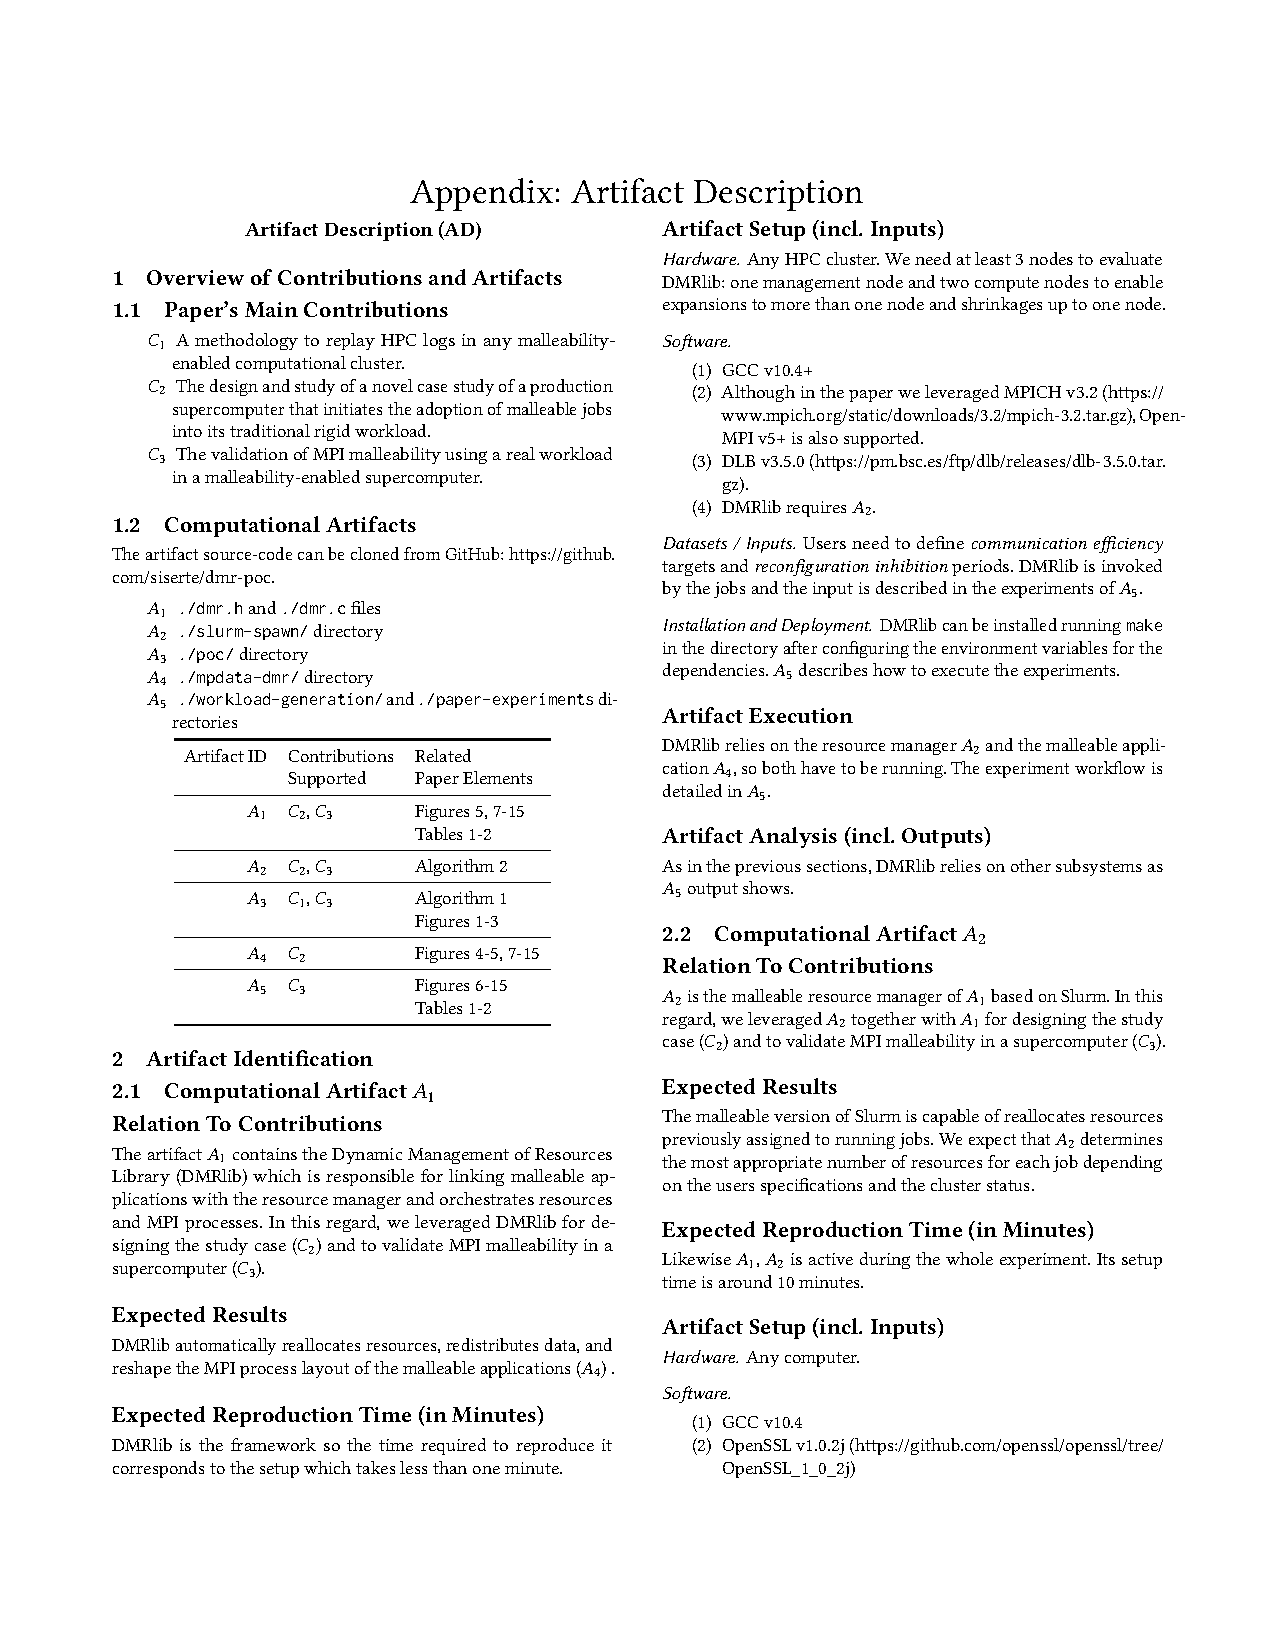
\includepdf[pages=-]{artifact.pdf}

\end{document}

